% MSc dissertation example file, February 2022
%
% Leave one of the documentclass lines uncommented to match your degree.
% You may remove the logo option if it causes problems.
% Do not change any other options.
% \documentclass[logo,msc,adi]{infthesis}     % Adv Design Inf
% \documentclass[logo,msc,ai]{infthesis}      % AI
% \documentclass[logo,msc,cogsci]{infthesis}  % Cognitive Sci
% \documentclass[logo,msc,cs]{infthesis}      % Computer Sci
% \documentclass[logo,msc,cyber]{infthesis}   % Cyber Sec
% \documentclass[logo,msc,datasci]{infthesis} % Data Sci
% \documentclass[logo,msc,di]{infthesis}      % Design Inf
% \documentclass[logo,msc,dsti]{infthesis}    % Data Sci TI
% \documentclass[logo,msc,inf]{infthesis}     % Informatics
\documentclass[logo,msc,inf]{infthesis}       % Informatics
%%%%%%%%%%%%%%%%%%%%%%%%
% Understand any problems and seek approval before assuming it's ok to remove ugcheck.
\usepackage{msccheck}
\usepackage{booktabs}  % \toprule, \midrule, \bottomrule
\usepackage{tabularx}  % tabularx and X columns
\usepackage{array}     % \arraybackslash
\usepackage{graphicx}
% Search the uploaded Overleaf figures folder first, then the project root.
\graphicspath{{figures/}{./}}
\usepackage{amsmath}
\usepackage[hyphens]{url}
\usepackage{placeins}  % keeps each Results figure with its RQ section
% UTF-8 input and CJK support for the verbatim multilingual prompt appendix.
\usepackage[utf8]{inputenc}
\usepackage{CJKutf8}
% Allow LaTeX extra freedom when choosing line breaks so that long tokens,
% identifiers, and URLs can wrap instead of overflowing the text width.
\emergencystretch=2em
% Include any packages you need below, but don't include any that change the page
% layout or style of the dissertation. By including the ugcheck package above,
% you should catch most accidental changes of page layout though.

% microtype omitted: it changes \showhyphens and triggers msccheck.

\begin{document}
\begin{preliminary}

\title{How Reliable Are LLMs as Cognitive Models? A Systematic
Evaluation of Prompt Sensitivity Across Decision-Making Tasks}

\author{Yijun Chen}

\date{\today}

\abstract{
Large language models (LLMs) are increasingly used to generate measurable experimental behaviour, yet the stability of behavioural conclusions drawn from a single prompt formulation has seldom been examined systematically across models, tasks, and languages. This study operationalises behavioural reliability as the robustness of task-specific conclusions to predefined prompt formulations when task rules and available information are held constant; behavioural similarity is not taken to imply shared human cognitive mechanisms. A Neutral baseline, Instruction specificity, Role framing, and Task-specific construct emphasis were compared in the Horizon Task, Iowa Gambling Task, and Balloon Analogue Risk Task. The English experiment included GPT-4.1, GPT-5.4, and GPT-5.4 Mini; the multilingual experiment fixed GPT-4.1 and analysed English, Simplified Chinese, and Spanish jointly as equally weighted conditions. Each model--language--task--prompt cell contained 20 complete runs, yielding 1,200 unique valid task runs. Analyses estimated raw prompt effects, model-by-prompt interactions, and centred three-language baseline and prompt-effect deviations across eight task-specific metrics. Uncertainty was represented by 2,000 task-appropriate bootstrap replicates, while human-reference proximity was assessed descriptively using human-SD-scaled mean deviations and empirical-interval coverage. Prompt formulations were associated with changes in several behaviours, but effect direction and magnitude varied by model, task, metric, and language implementation; no consistent formulation ranking emerged. Human-reference proximity also changed in some cells, and mean deviation did not invariably track interval coverage. The answer to the title question is therefore conditional: the tested LLMs cannot be treated as reliably prompt-invariant cognitive models, although they can support reproducible measurement of cognitive-task behaviour when the complete measurement specification is fixed, reported, and evaluated for robustness. The principal contribution is an auditable, reviewable multi-task evaluation framework, not evidence of mechanistic or distributional equivalence between LLM runs and human participants.
\par\medskip\noindent\textbf{Keywords:} large language models; prompt sensitivity; behavioural reliability; decision-making tasks; cross-language evaluation; human-reference comparison
}

\maketitle

\newenvironment{ethics}
   {\begin{frontenv}{Research Ethics Approval}{\LARGE}}
   {\end{frontenv}\newpage}

\begin{ethics}
This project was planned in accordance with the Informatics Research
Ethics policy. It did not involve any aspects that required approval
from the Informatics Research Ethics committee.

\standarddeclaration
\end{ethics}


\begin{acknowledgements}
I would like to thank my supervisor, Bonan Zhao, for her guidance, feedback,
and support throughout this project.
\end{acknowledgements}


\tableofcontents
\end{preliminary}


\chapter{Introduction}

LLMs are increasingly studied as behavioural systems. They have been used to simulate respondents and reproduce selected experimental effects \cite{Argyle2023OutOfOneMany,Aher2023SimulateHumans}. Other work has treated them as economic agents \cite{Horton2023HomoSilicus} or examined their performance on cognitive tasks \cite{Binz2023CognitivePsychologyGPT3,Hagendorff2023HumanLikeBiases}. Their responses can be generated repeatedly under controlled task manipulations, but one run is not a human participant and behavioural similarity does not establish a shared mechanism. Here, \emph{cognitive model} means a computational model that produces measurable behaviour in cognitive tasks, not a system assumed to share human cognition.

An LLM output is conditional on its input and generation settings. Prompts can assign a role, alter salience, and constrain responses; formulation and temperature can change task behaviour \cite{Loya2023PromptSensitivityDecision}. Reliability must therefore include whether task-specific conclusions survive prespecified formulations that preserve task rules and available information. Divergent exploration, learning, or risk-taking under such formulations indicates dependence on the measurement procedure, even when each response remains interpretable.

Multi-template evaluations have mainly examined static benchmarks and formatting changes \cite{Sclar2024PromptFormatting}; the sequential Horizon study of Loya et al.~\cite{Loya2023PromptSensitivityDecision} covered one paradigm. Existing evidence therefore does not establish whether conclusions remain stable across full task runs, controlled prompt variants, models, tasks, metrics, and languages while keeping behavioural outcomes distinct from human-reference proximity. These dimensions are not interchangeable: a model may be stable but unlike the reference sample, or human-proximal only under one prompt.

Multilingual performance also varies across languages and tasks \cite{Ahuja2023MEGA}. Cross-language behavioural comparison therefore requires a fixed model and task environment plus aligned task information and manipulation intent, without claiming complete pragmatic equivalence.

The Horizon Task, IGT, and BART respectively examine exploration, adaptation to reward--loss feedback, and sequential risk-taking \cite{Wilson2014,Bechara1994,Lejuez2002}. Available participant-level datasets permit descriptive comparison with aligned LLM run summaries \cite{Feng2021ExploreExploit,Steingroever2015IGTData,Sebri2023BART}, but proximity is not evidence of shared mechanisms.

The study compares a Neutral baseline with Instruction specificity, Role framing, and Task-specific construct emphasis while preserving actions, feedback, and hidden-information boundaries. English runs compare GPT-4.1, GPT-5.4, and GPT-5.4 Mini; the multilingual analysis fixes GPT-4.1 and jointly compares English, Simplified Chinese, and Spanish.

The contribution is an auditable framework that (i) defines robustness across task-rule-matched formulations, (ii) estimates task- and metric-specific model-by-prompt differences, (iii) separates behavioural outcomes from human-reference proximity, and (iv) locates three languages symmetrically in a common centred coordinate system. Construct emphasis is a substantive salience manipulation, so its effect is not automatically classified as instability due to incidental wording.

The study addresses the following research questions:

\noindent\textbf{RQ1 --- Prompt sensitivity.}
To what extent do Instruction specificity, Role framing, and Task-specific construct emphasis alter a model's task-specific behaviour relative to the Neutral baseline?

\noindent\textbf{RQ2 --- Cross-model variation.}
Within each task and behavioural metric, do the prompt effects of GPT-4.1 or GPT-5.4 Mini differ from those of GPT-5.4? Do the directions and magnitudes of these differences exhibit recurring descriptive patterns across tasks and metrics?

\noindent\textbf{RQ3 --- Cross-language variation.}
When the model, task environment, and generation parameters are held constant, and the intended prompt manipulations and task-relevant information are semantically aligned across languages, do English, Simplified Chinese, and Spanish produce different baseline behaviours or within-language prompt effects?

\noindent\textbf{RQ4 --- Prompt-associated changes in human-reference proximity.}
Relative to the Neutral baseline, do alternative prompt formulations change the absolute human-SD-scaled mean deviation from the human reference mean or the proportion of runs falling within the empirical human reference interval?

RQ4 is descriptive: each condition and Neutral are located against the same fixed human reference. Human-SD-scaled deviations and empirical coverage are not Cohen's \(d\), significance tests, or evidence of shared mechanisms.

Prompt effects varied in direction and magnitude across models, tasks, metrics, and languages; no formulation ranked consistently. Cross-model interactions, centred three-language comparisons, and changes in human-reference deviation and coverage show that conclusions from one prompt, model, or language do not automatically generalise. LLMs are therefore conditionally reliable models of cognitive-task behaviour under a complete measurement specification, not prompt-invariant models of human cognition.

Background positions the study in prior behavioural, prompt-robustness, multilingual, and decision-task research. Method defines the design and analyses; Results addresses RQ1--RQ4; Discussion interprets their methodological implications and limits; Conclusions answers the central question and identifies priorities for future work.

\chapter{Background and Related Work}
\section{LLMs as Behavioural Subjects and Computational Models}
LLMs have been used to simulate human participants, an application that requires valid population inference \cite{Dillion2023ReplaceParticipants}. A distinct machine-behaviour tradition instead treats artificial systems as experimental subjects to be characterised in their own right \cite{Rahwan2019MachineBehaviour,Hagendorff2023MachinePsychology}. This study adopts the latter position and defines an LLM operationally as a model producing measurable cognitive-task behaviour, without assuming human perceptual, learning, or decision mechanisms \cite{Lin2025SixFallacies}.

Coherent agent behaviour can depend on surrounding memory, reflection, and planning components \cite{Park2023GenerativeAgents}, while synthetic responses may compress human heterogeneity or change correspondence when the model or prompt changes \cite{Dillion2023ReplaceParticipants,Bisbee2024SyntheticSurveyData}. The object of study is therefore the model--task--measurement system, not a substitute human population.

\section{Reliability in the Behavioural Measurement of LLMs}

Behavioural evaluation concerns distributions and trajectories as well as accuracy. Multi-template studies show that conclusions drawn from one prompt can be unstable \cite{Sclar2024PromptFormatting,Mizrahi2024MultiPrompt}. Separate work demonstrates that evaluation and scoring artefacts can themselves create apparent variation \cite{Hua2025FlawArtifact}. Here, \emph{behavioural-measurement reliability} means stability in a conclusion's direction and magnitude across prespecified formulations with model snapshot, task, temperature, response format, and parser fixed. It excludes long-term test--retest reliability, external validity, and claims about mechanisms.

Prompt wording and formatting form part of the measurement procedure \cite{Sclar2024PromptFormatting}; in sequential tasks, visible history and interface design also condition behaviour \cite{Loya2023PromptSensitivityDecision}. Temperature, parser rules, and deployment state add further implementation dependence, while proprietary updates can change behaviour over time \cite{Chen2024ChatGPTBehavior}. Fixing the parser reduces ambiguity but not effects of length, salience, or position. Complete runs are analytical replicates, not independent synthetic persons, because they share parameters and deployment conditions \cite{Dillion2023ReplaceParticipants,Bisbee2024SyntheticSurveyData}. Prompt stability, task-specific outcomes, and human-reference proximity are therefore reported separately: stability is not quality, and mean proximity is not distributional or mechanistic equivalence \cite{Lin2025SixFallacies}.

\section{Prompt Sensitivity and Behavioural Variation}

Output probabilities can depend on label choice and demonstration order \cite{Zhao2021Calibrate,Lu2022PromptOrder}. Formatting and option order introduce additional variation \cite{Sclar2024PromptFormatting,Pezeshkpour2024OptionOrder}, while high scores can persist under semantically misleading instructions \cite{Webson2022PromptMeaning}. Multi-prompt evaluation therefore replaces the search for one best prompt \cite{Mizrahi2024MultiPrompt,Zhuo2024ProSA}, but most evidence is static; Loya et al.~\cite{Loya2023PromptSensitivityDecision} examined one sequential task without multilingual comparison.

Manipulation type matters. Formatting tests incidental sensitivity, whereas role-play can alter reasoning performance \cite{Kong2024RolePlayPrompting}. Instruction specificity, Role framing, and Task-specific construct emphasis may change rule representation, role context, or salience. Because they also differ in length, keywords, and position, inference concerns the whole formulation; these correlated features cannot be decomposed retrospectively, and an effect is not automatically instability caused by irrelevant wording \cite{Sclar2024PromptFormatting,Hua2025FlawArtifact}.

\section{Model Variation and Reproducibility in LLM Measurement}

Prompt robustness studies report variation between models as well as between formulations \cite{Sclar2024PromptFormatting,Mizrahi2024MultiPrompt}. ProSA similarly treats sensitivity as model- and prompt-dependent rather than as a property of a single template \cite{Zhuo2024ProSA}. Comparing one-condition means cannot separate baseline variation from response to formulation; the appropriate contrast first estimates each model's condition-minus-Neutral effect and then compares effects directly.

Proprietary versions may also change opaquely, so a model name does not guarantee identical behaviour across dates \cite{Chen2024ChatGPTBehavior,Palmer2024ProprietaryModels}. This study records resolved identifiers, dates, settings, prompt versions, and failures, but restricts inference to tested snapshots and does not attribute differences causally to architecture or scale.

\section{Language Effects in LLM Behavioural Measurement}

Multilingual capability is not a proportional replication of English performance: accuracy and cultural knowledge vary by language, task, and model, and higher average performance need not mean greater consistency \cite{Zhang2023M3Exam,Qi2023CrossLingualConsistency}. Transfer from English instruction tuning depends on coverage, format, demonstrations, reasoning strategy, and which prompt components are translated \cite{Muennighoff2023CrosslingualGeneralization,Shi2023MultilingualCoT,Mondshine2025BeyondEnglish}. Fewer studies compare both baselines and within-language prompt effects in full behavioural runs.

Translation is therefore part of the experiment. Task-relevant informational equivalence does not guarantee equal naturalness, pragmatics, salience, or measurement properties. Results are described as language-associated differences conditional on the tested model, translations, and task implementation.


\section{Sequential Decision Tasks and Their Cognitive Constructs}

In the Horizon Task, IGT, and BART, choices and feedback form within-run trajectories \cite{Wilson2014,Bechara1994,Lejuez2002}. Sequential LLM experiments likewise require histories to remain grouped within complete runs \cite{Loya2023PromptSensitivityDecision}. The complete run is therefore the analysis unit rather than treating trials as independent participants.

The Horizon Task uses information asymmetry and the number of remaining decision opportunities to examine the explore--exploit dilemma \cite{Wilson2014}. Directed and random exploration can produce superficially similar choices while corresponding to different computational descriptions \cite{Gershman2018Exploration}. The information-seeking choice rate, horizon-related exploration change, and model-derived decision-noise difference should therefore be interpreted separately.

The original IGT operationalises learning through repeated deck choices and feedback \cite{Bechara1994}. Computational accounts show that the same deck preference may arise from different valuation, learning, and consistency processes \cite{Busemeyer2002PVL,Steingroever2013PVLDelta}; construct-validity reviews therefore caution against a unitary ability score \cite{Buelow2009IGTValidity}. Recent cognitive-modelling work has likewise decomposed LLM choices in an adapted Iowa Gambling Task into valuation, learning, and consistency components \cite{Yang2026IrrationalAgent}. Explicit cumulative information may also reduce LLM memory demands, so interpretation is limited to aligned metrics.

The original BART uses pumping behaviour as an operational measure of risk taking \cite{Lejuez2002}. Later modelling work shows that pumps can also reflect learning and response consistency \cite{Wallsten2005BARTModel,VanRavenzwaaij2011BART}; adjusted pumps, explosions, and post-explosion adjustment are therefore complementary. LLM implementations of these tasks have additionally been used to study gambling-like risk-taking, with interventions motivated by behavioural economics rather than by cognitive modelling \cite{Du2025GamblingRisk}. Because task constructs, scales, and feedback differ, no cross-task ``decision-making ability'' score is constructed.

\section{Human-Reference Comparisons: Purpose and Limits}

Human-reference comparisons distinguish mean position, empirical-interval coverage, and response to manipulation. These answer different questions: similar aggregate output does not imply identical task behaviour or mechanism \cite{Lin2025SixFallacies}. An LLM run can align operationally with a participant summary but is not an independent human; task length, presentation, and familiarisation further constrain comparison \cite{Dillion2023ReplaceParticipants,Bisbee2024SyntheticSurveyData}. Direct comparisons of LLMs with human decision-makers on the same tasks likewise report near-optimal choices alongside non-human learning dynamics \cite{Li2025NearOptimal}.

The reference is not a normative target: neither BART pumps nor information seeking has a context-independent optimum. Signed and absolute human-SD-scaled mean deviation and coverage are complementary descriptive quantities, not Cohen's \(d\), distributional equivalence, performance rankings, or evidence of shared mechanisms.

\section{Research Gap and Positioning of the Present Study}

Synthetic-participant and machine-psychology studies pursue different inferential objectives \cite{Dillion2023ReplaceParticipants,Hagendorff2023MachinePsychology}. Prompt-robustness research focuses primarily on measurement variation \cite{Mizrahi2024MultiPrompt}, while multilingual benchmarks examine language coverage and performance \cite{Zhang2023M3Exam}. These strands do not jointly evaluate measurement stability, task-specific behaviour, and human-reference proximity. Existing multi-prompt evidence remains concentrated in static benchmarks \cite{Sclar2024PromptFormatting}; the principal sequential extension covers one task \cite{Loya2023PromptSensitivityDecision}, and multilingual consistency studies use other benchmark settings \cite{Qi2023CrossLingualConsistency}.

Within the reviewed literature, no identified design combines full sequential runs, controlled prompt variants, multiple models and decision constructs, and a fixed-model multilingual comparison. Recent LLM decision-making studies focus on optimality or safety rather than on measurement robustness \cite{Li2025NearOptimal,Du2025GamblingRisk}, and cognitive-modelling analyses of LLM choices on the Iowa Gambling Task do not compare behaviour across prompt formulations \cite{Yang2026IrrationalAgent}. The present design extends sequential prompt-sensitivity work \cite{Loya2023PromptSensitivityDecision} with the multi-formulation logic used in broader robustness evaluations \cite{Sclar2024PromptFormatting,Mizrahi2024MultiPrompt}. It tests whether cognitive-task conclusions remain robust, not whether LLMs are globally human-like.

\chapter{Methodology}

\section{Study Design and Scope}

The controlled repeated-run design held task rules, environment, and available information constant. An English three-model comparison tested model variation; a GPT-4.1 three-language comparison tested aligned English, Simplified Chinese, and Spanish baselines and prompt effects.

Each model completed Horizon, IGT, and BART under Neutral, Instruction specificity, Role framing, and Task-specific construct emphasis. Each comparison contained $3\times3\times4\times20=720$ runs. Because 240 English GPT-4.1 runs were shared rather than replicated, the deduplicated total was 1,200 (Figure~\ref{fig:study_design_scope}).

The shared English GPT-4.1 sample links the two comparisons but is not an independent replication. Incomplete runs were replaced under the same technical criteria until every cell reached its prespecified target; wide intervals were treated as imprecision rather than evidence that a prompt effect was absent.

\begin{figure}[htbp]
\centering
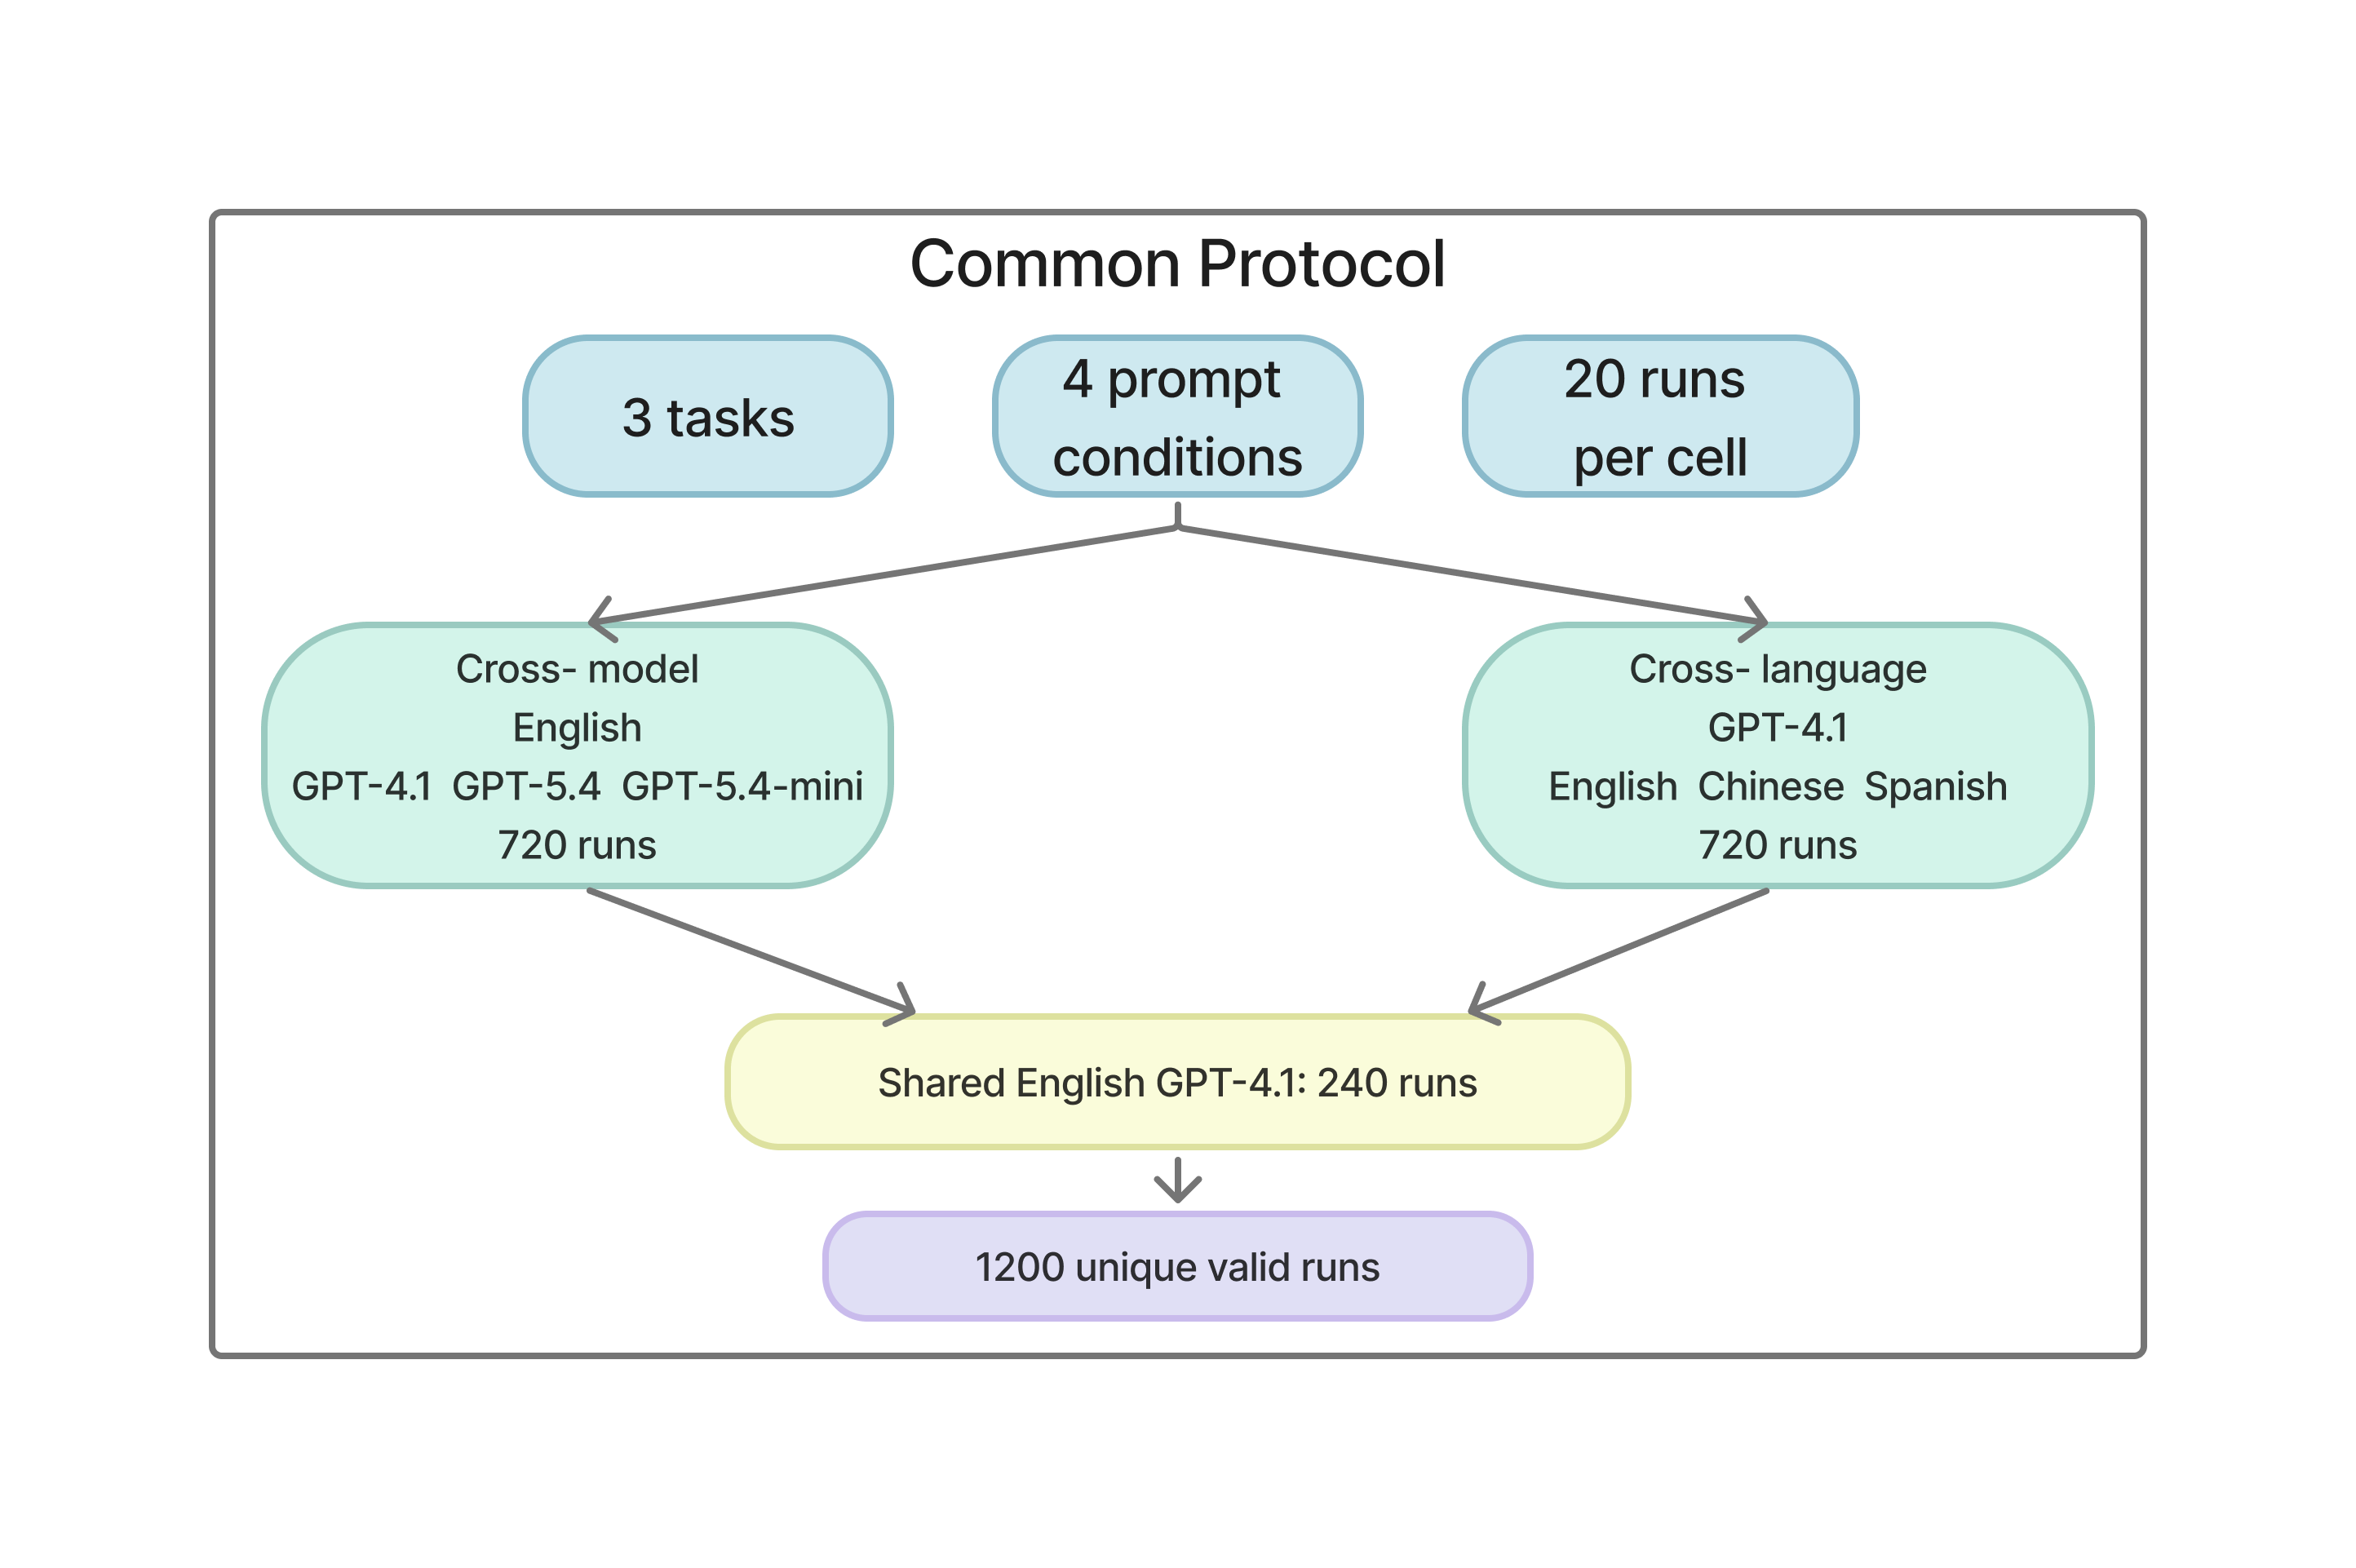
\includegraphics[width=0.98\textwidth]{study_design_scope.png}
\caption{Study design and deduplicated data structure. The shared English GPT-4.1 sample is counted once.}
\label{fig:study_design_scope}
\end{figure}

Twenty valid runs per cell reflected the computational budget rather than a formal power calculation: the full $3\times3\times4$ factorial structure at this cell size kept each comparison arm at 720 runs and the deduplicated total at 1,200, while bounding API cost and collection time, because larger cells would have scaled both linearly without a prespecified precision target. Bootstrap intervals are therefore reported as the primary expression of uncertainty precisely because 20 runs per cell cannot by themselves support narrow inference. Fixed criteria replaced technical failures but retained behavioural extremes and zero variance. Complete runs were the statistical units, with trials nested within them, and served only as participant-level analogues for aligned description.

Prompt sensitivity denotes change from same-model Neutral when rules, actions, feedback, and hidden-information boundaries remain fixed. Effects concern each complete formulation: specificity expands rules, framing changes role context, and construct emphasis changes salience. Reliability means robustness of task-specific conclusions across these formulations, not better performance, human likeness, or complete pragmatic equivalence across languages.

This factorial structure separates three questions that a single-prompt evaluation would conflate. Within-model contrasts estimate sensitivity to formulation under a fixed model snapshot; model-by-prompt contrasts test whether that sensitivity generalises across systems; and the symmetric language analysis asks whether baseline location and prompt response occupy comparable positions across language implementations. Repeated complete runs estimate variation in generated task trajectories, but they do not constitute independent members of a synthetic population or repeated measurements of a persistent agent.

\section{Models and API Configuration}

Models were accessed through the University of Edinburgh ELM platform's OpenAI-compatible Responses API. GPT-4.1, GPT-5.4, and GPT-5.4 Mini tested variation in prompt sensitivity, not capability rankings; undisclosed architecture or training differences were not inferred.

All models used identical task implementations, prompt conditions, response constraints, and repeated-run procedures. Generation settings were \texttt{temperature} = 0.7, \texttt{top\_p} = 1.0, and \texttt{max\_output\_tokens} = 16. GPT-5.4 and GPT-5.4 Mini used \texttt{reasoning\_effort} = none; GPT-4.1 used its standard non-reasoning configuration. The ELM API did not expose a controllable token-sampling seed. Task-environment seeds therefore controlled environmental randomisation, but not model-generation randomness.

\begin{table}[htbp]
\centering
\caption{Model identifiers and formal data-collection periods.}
\label{tab:model_identifiers}
\begin{tabularx}{\textwidth}{@{}>{\raggedright\arraybackslash}p{2.5cm}>{\raggedright\arraybackslash}X>{\raggedright\arraybackslash}X@{}}
\toprule
\textbf{Model and scope} & \textbf{Resolved identifier} & \textbf{Collection period} \\
\midrule
GPT-4.1 (three languages) & \texttt{gpt-4.1-2025-04-14} & English: 8--13 July 2026\newline Chinese: 3--5 August 2026\newline Spanish: 5--7 August 2026 \\
GPT-5.4 (English) & \texttt{gpt-5.4-2026-03-05} & 30--31 July 2026 \\
GPT-5.4 Mini (English) & \texttt{gpt-5.4-mini-2026-03-17} & 1 August 2026 \\
\bottomrule
\end{tabularx}
\end{table}

Dates are formal output-generation dates in the Asia/Shanghai time zone. GPT-4.1 data were collected in separate language batches; possible provider-side temporal drift is addressed under Reproducibility.

\section{Decision-Making Tasks}

Three sequential tasks examined exploration--exploitation, feedback-based learning, and risk-taking. At each step, the model received the current state and feedback and selected a constrained action; hidden parameters and future outcomes remained unavailable.

The tasks were selected because they impose different temporal and informational demands while yielding interpretable behavioural summaries. Horizon isolates first-free-choice responses to reward and information asymmetry; IGT requires learning from repeated gains and losses under a fixed payoff structure; and BART couples incremental reward with an increasing chance of losing the temporary return. Their differences make agreement across tasks informative, while also preventing raw scores from being collapsed into a single cross-task performance measure.

\subsection{Horizon Task}

Each Horizon run contained 40 two-option games \cite{Wilson2014}. Four forced choices preceded a single free choice in H1, and the same four forced choices preceded six free choices in H6. The model saw game and choice numbers, choices remaining, reward history, and any forced option, but not internal condition labels.

Equal-information games forced two observations per option; unequal games forced one versus three, with option identity and forced order randomised. The four horizon-by-information combinations each occurred ten times in fixed balanced order. Seeds controlled option assignment, forced order, latent means, and rewards, not condition counts.

Latent option means were an anchor in $\{40,60\}$ and that anchor plus a non-zero difference in $\{-30,-20,-12,-8,-4,4,8,12,20,30\}$, randomly assigned to A/B. Rewards were Gaussian (SD 8), integer-rounded and clipped to $[1,100]$; means were hidden. Matched seeds reproduced potential sequences, although different choices could yield different observed histories.

\subsection{Iowa Gambling Task}

IGT comprised 100 choices from an initial 2,000 points \cite{Bechara1994}. Decks A/B paid 100 and C/D 50 before deterministic ten-selection loss cycles; A/B netted $-250$ and C/D $+250$ per cycle. A/C had frequent losses and B/D rarer, larger losses.

Long-run properties were hidden. Observations reported the last outcome, total, deck counts, cumulative and mean net outcomes, and five recent trials. These aids reduce memory demand relative to the human task, so comparisons cover aligned choices only. Trials were continuous with no reset or environmental randomisation.

\subsection{Balloon Analogue Risk Task}

BART contained 40 balloons in two recording blocks \cite{Lejuez2002}. Each successful \texttt{PUMP} added 0.05; \texttt{CASH\_OUT} banked the temporary value, whereas explosion forfeited it.

Explosion points were generated from the environment seed at run initialisation. At pump $k$,
\[
P(\text{explosion at pump }k\mid\text{survival through pumps }1,\ldots,k-1)=\frac{1}{33-k}
\]
for $k=1,\ldots,32$; explosion was certain at pump 32. The model knew only that risk increased and balloons could differ; it saw the current count and value, total, previous and five recent outcomes, cumulative explosions, and mean pumps. Seeds fixed 40 latent explosion points.

\section{Prompt Construction and Validation}

\subsection{Prompt Conditions}

Neutral contained only necessary rules, actions, and response requirements. Instruction specificity expanded the same rules; Role framing requested a human-participant role without a strategy; construct emphasis highlighted Horizon uncertainty, IGT reward/loss, or BART risk without revealing hidden parameters or prescribing choices.

Rules, feedback, payoff, task length, response format, and hidden-information boundaries were fixed in independent contexts. Length was not artificially matched, and unverifiable public-tokeniser estimates were not used as covariates. Effects therefore concern the full formulation, not isolated length, repetition, position, or keywords.

The variants were designed as controlled measurement implementations rather than attempts to optimise performance. Instruction specificity clarified already available information; Role framing changed the requested perspective; and construct emphasis altered the salience of a task-relevant concept. Because these manipulations necessarily differ in wording, length, position, and keyword salience, their estimated effects cannot be attributed to a single linguistic feature; this is a design limitation rather than a nuisance, and the inferential object is therefore the complete prespecified formulation relative to its task-matched Neutral baseline, not an isolated causal effect of role, specificity, or emphasis.

\subsection{Prompt Provenance, Validation, and Freezing}

Three literature-based baselines and nine constrained variants were checked for task information, response format, manipulation fidelity, unintended disclosure, and strategy advice. Pretesting established parser compatibility; materials were then frozen. Appendix~\ref{app:materials} records the prompt inventory and provenance trail; the complete verbatim prompt texts are reproduced in Appendix~\ref{app:prompts}.

\subsection{Multilingual Prompt Construction and Validation}

English was the source for 12 Chinese and 12 Spanish task--condition prompts. A common checklist and AI-assisted review screened omissions, additions, manipulation drift, numerical rules, hidden-information boundaries, and response formats; the researcher made final decisions. Action labels and parameters were identical, but no independent bilingual review or back-translation was conducted. The procedure supports task-relevant informational, not complete pragmatic or cultural, equivalence.

Both static instructions and dynamically generated observations were presented in the target language. All language materials were frozen before collection, so later review did not alter the prompts used to produce the formal data.

\section{Experimental Procedure and Data Quality}

Figure~\ref{fig:experimental_workflow} shows the conversion of a planned cell into a complete run. The manifest identified its model, language, task, prompt condition, and environment seed; task and condition keys selected the corresponding frozen language prompt and instantiated the Horizon, IGT, or BART environment.

\begin{figure}[htbp]
\centering
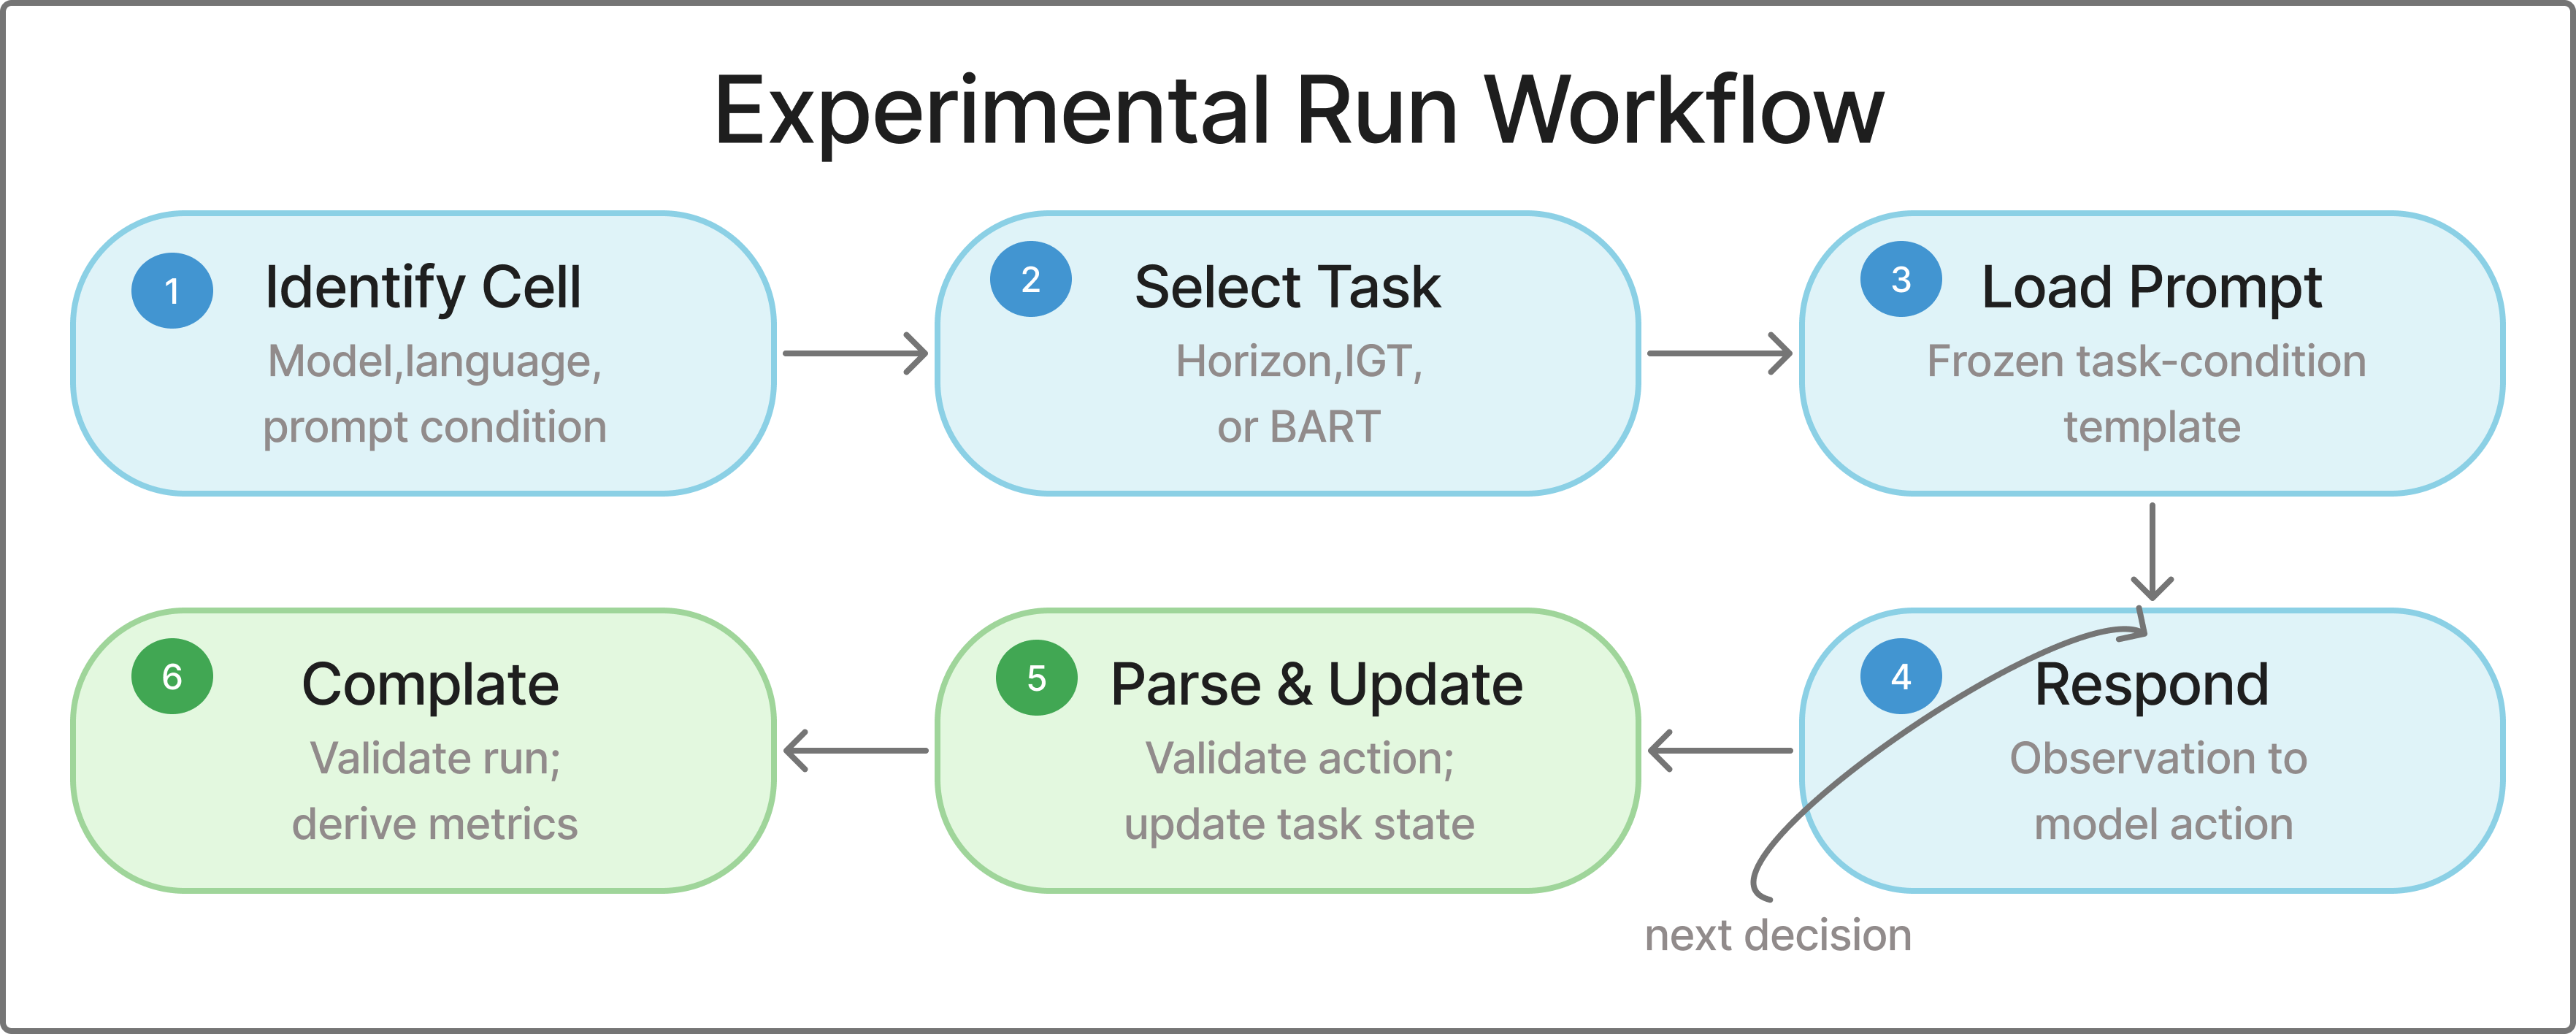
\includegraphics[width=0.98\textwidth]{experimental_workflow.png}
\caption{Experimental workflow from frozen materials to formal analysis.}
\label{fig:experimental_workflow}
\end{figure}

\subsection{Run Procedure}

The cross-model experiment targeted 20 valid runs per model--task--condition cell; the multilingual experiment fixed GPT-4.1 and retained the task, condition, and base-seed structure across languages. Each run used an independent context. At every decision, the runner inserted the current state and deterministic history into the frozen template, submitted one request, parsed the response, and updated the environment only after a valid action. This loop continued to the task endpoint without persistent conversation or model-generated summaries. Context length varied with task histories and prompt length.

Horizon and BART seeds aligned initial environments across models, conditions, and languages, although realised feedback could diverge after different choices. IGT used a fixed payoff schedule, so its nominal seed identified corresponding runs but did not support paired-seed inference. Environmental seeds did not control token sampling because the API exposed no generation seed.

Full task runs, rather than individual trials, formed the replication units because decisions within a run shared an evolving history. This preserved adaptation to earlier outcomes and prevented later trials from being treated as independent observations. It also means that matched environmental seeds align opportunities for comparison without guaranteeing identical realised histories once models choose different actions.

\subsection{Response Parsing and Quality Control}

The parsers accepted only the task's response vocabulary: \texttt{CHOICE: A/B} for Horizon, \texttt{CHOICE: A/B/C/D} for IGT, and \texttt{ACTION: PUMP/CASH\_OUT} for BART. Matching was case-insensitive and allowed surrounding whitespace or a complete Markdown code fence, but never inferred an action from explanatory prose. An initial parse failure triggered one identical repeat request without advancing the state; a second failure or unrecoverable service error marked the run incomplete. Formal analysis required the planned configuration and a complete response, action, and state history. Successfully retried runs remained eligible, whereas technically incomplete runs were replaced independently of their behavioural direction or extremity.

\section{Human Reference Data}

One existing dataset per task provided a descriptive, non-normative reference. Selection required adequate task comparability, trial-level records for the primary metrics, and participant-level summaries. Feng et al.~\cite{Feng2021ExploreExploit} supplied 60 complete Horizon participants (320 games per participant, compared with 40 games per LLM run); Steingroever et al.~\cite{Steingroever2015IGTData} supplied 504 healthy participants with 100 complete IGT trials; and Sebri et al.~\cite{Sebri2023BART} supplied 141 adults after excluding six minors (140 for post-explosion adjustment). Human BART matched the 40 balloons, 0.05 increment, and explosion schedule but included familiarisation absent from the LLM task. Human records were converted to participant summaries using the LLM metric definitions. Comparisons were restricted to alignable measures and did not pool participants across tasks or equate measurement precision.

These datasets were used to locate LLM cell means and run-level values relative to fixed empirical benchmarks, not to define normative performance. Differences in recruitment, instructions, familiarisation, task presentation, and sample size remain part of the comparison. Accordingly, human-reference results are conditional on the selected datasets and aligned metrics and do not imply that an LLM run is exchangeable with a human participant.

\section{Statistical Analysis}

\subsection{Behavioural Metrics}

Eight primary behavioural metrics were analysed. Seven were calculated directly
from each complete run, whereas the eighth---the Random exploration effect---was
estimated jointly within each model--language--prompt cell using a first-free-choice
hierarchical logistic choice model. This model produced one cell estimate and
partially pooled run-level estimates.

\begin{table}[htbp]
\centering
\caption{Primary behavioural metrics.}
\label{tab:behavioural_metrics}
\begin{tabularx}{\textwidth}{@{}p{1.7cm}p{3.8cm}X@{}}
\toprule
\textbf{Task} & \textbf{Metric} & \textbf{Operational definition} \\
\midrule
Horizon & Information-seeking choice rate & Proportion of first free choices in unequal-information games on which the less-observed option was chosen. \\
Horizon & Horizon-related\newline exploration change & H6 minus H1 exploratory-choice rate; pre-choice mean ties excluded. \\
Horizon & Random exploration effect & H6 minus H1 model-estimated decision noise. \\
IGT & Advantageous choice rate & Proportion of choices from decks C or D. \\
IGT & Post-loss switching rate & Deck switch after a negative loss component. \\
BART & Adjusted average pumps & Mean pumps on non-exploded balloons. \\
BART & Explosion rate & Proportion of balloons that exploded. \\
BART & Post-explosion\newline adjustment & Pumps on the next balloon minus pumps on the exploded balloon. \\
\bottomrule
\end{tabularx}
\end{table}

Adjusted pumps conditions on balloon survival and was therefore interpreted with explosion rate. Information-seeking rate is a level measure, not the classic horizon-dependent directed-exploration effect: it was defined on first free choices in unequal-information games, where a less-observed option exists. For run $i$, let $E_{i,h}$ denote the proportion of eligible first free choices selecting the option with the lower pre-choice observed mean at horizon $h$; eligibility required both pre-choice observed means to be defined and unequal, and first free choices from both equal- and unequal-information games contributed. The horizon-related change was
\[
\mathrm{HorizonEffect}_{i}=E_{i,\mathrm{H6}}-E_{i,\mathrm{H1}}.
\]
It was missing if either horizon had no eligible choice. In IGT, a loss event required the signed \texttt{loss} field to be negative, irrespective of net outcome; switching was evaluated on the following trial, so trial 100 was ineligible. Post-explosion adjustment was missing when no explosion had a subsequent balloon.

Random exploration used only the first free choice. For the probability $p_{i,g,h}$ that run $i$ selected A in game $g$ at horizon $h$,
\[
\begin{aligned}
\operatorname{logit}(p_{i,g,h})&=\beta_{i,h}(\Delta R_{ig}+\gamma_h\Delta I_{ig}+\delta_h),\\
\beta_{i,h}&=\exp(\alpha_h+u_{i,h}),\qquad \sigma_{i,h}=1/\beta_{i,h},\\
\mathrm{RE}_{i}&=\sigma_{i,\mathrm{H6}}-\sigma_{i,\mathrm{H1}}.
\end{aligned}
\]
$\Delta R_{ig}$ is the A-minus-B observed mean reward in game $g$; $\Delta I_{ig}$ is 1 when A is less observed, $-1$ when B is less observed, and 0 otherwise. $\gamma_h$ is the information bonus and $\delta_h$ the label bias, while $u_{i,h}$ is the run-level random effect with Gaussian shrinkage. Although the code names $\beta$ reward sensitivity, it scales the complete evidence expression and acts as inverse temperature. The cell estimate used $\beta_h^{*}=\exp(\alpha_h)$; run summaries used the jointly estimated, partially pooled $\mathrm{RE}_i$. Positive RE denotes greater estimated choice variability at H6, not proof of psychological randomness. Read concretely, the model scores each option from the observed evidence---past rewards, an information bonus for the less-observed option, and a label bias---and $\beta_{i,h}$ controls how consistently choices follow that score; because $\sigma_{i,h}=1/\beta_{i,h}$, the random-exploration effect asks whether estimated decision noise is higher at H6 than at H1, that is, whether a longer decision horizon increases choice variability beyond what the observed evidence alone predicts. MAP estimation used Gaussian run-effect shrinkage (primary SD 0.5; sensitivity 0.25 and 1.0), and relevant bootstrap replicates refitted the model. All sensitivity fits converged, but the estimated random-exploration magnitudes changed with the shrinkage scale, so the main text treats this latent estimate as model-dependent rather than as a precise point estimate. Implementation-level fit and optimiser diagnostics are included in the repository materials indexed in Appendix~\ref{app:supplementary-results}.

\subsection{Prompt Effects}

For every cell, the valid $n$, mean, SD, median, range, and distribution were reported. For model $m$, language $\ell$, task $t$, manipulated condition $c$, and metric $k$, $\Delta_{m,\ell,t,c,k}$ was the manipulated-condition run mean minus the corresponding Neutral mean ($c=0$). This signed raw difference was primary. Standardised effects used
\[
g_{m,\ell,t,c,k}=J\frac{\bar Y_{m,\ell,t,c,k}-\bar Y_{m,\ell,t,0,k}}{s_{\mathrm{pooled}}},
\]
where $J$ is the conventional small-sample correction based on the combined degrees of freedom. Positive values indicate an increase in the metric, not necessarily improved performance. If $s_{\mathrm{pooled}}=0$, $g$ was undefined. Equal constants yielded a raw difference of zero and missing $g$ (\texttt{constant\_equal}); unequal constants yielded their raw difference and missing $g$ (\texttt{constant\_unequal}). Zero-SD bootstrap estimates were invalid rather than replaced with zero. Raw contrasts were always retained.

\subsection{Cross-Model Comparisons}
English was fixed and GPT-5.4 was prespecified as the reference. GPT-4.1 versus GPT-5.4 described earlier-versus-newer flagship differences; GPT-5.4 Mini versus GPT-5.4 described compact-versus-full-model differences. For $m\in\{\mathrm{GPT\mbox{-}4.1},\mathrm{GPT\mbox{-}5.4\ Mini}\}$,
\[
I^{\mathrm{model}}_{m,t,c,k}=\Delta_{m,\mathrm{en},t,c,k}-\Delta_{\mathrm{GPT\mbox{-}5.4},\mathrm{en},t,c,k}.
\]
Positive values indicate a more positive condition-minus-baseline effect for $m$ than GPT-5.4, not better performance. Raw interactions in original units were primary; within-model Hedges' $g$ described standardised magnitudes. Interpretation used magnitude, direction, and bootstrap 95\% intervals, without a causal difference-in-differences claim. Heterogeneous constructs and scales were not combined in an omnibus cross-task test.

\subsection{Cross-Language Comparisons}

GPT-4.1 was fixed, and English, Simplified Chinese, and Spanish were analysed jointly with equal status. English was the translation source, not the statistical reference. With $\mathcal L=\{\mathrm{en},\mathrm{zh\mbox{-}CN},\mathrm{es}\}$,
\[
B^{\mathrm{centred}}_{\ell,t,k}=\bar Y_{\mathrm{GPT\mbox{-}4.1},\ell,t,0,k}-\frac13\sum_{j\in\mathcal L}\bar Y_{\mathrm{GPT\mbox{-}4.1},j,t,0,k},
\]
and
\[
I^{\mathrm{centred}}_{\ell,t,c,k}=\Delta_{\mathrm{GPT\mbox{-}4.1},\ell,t,c,k}-\frac13\sum_{j\in\mathcal L}\Delta_{\mathrm{GPT\mbox{-}4.1},j,t,c,k}.
\]
The three deviations sum to zero for each task, metric, and condition. Positive values denote a baseline mean or prompt effect above the three-language mean, not better performance. Raw centred deviations were primary. Figures additionally show pooled-SD-scaled baseline deviations and each language's Hedges' $g$ centred on the three-language mean; the latter is not a conventional standardised regression interaction. Horizon and BART uncertainty retained matched environmental seeds; IGT independently resampled whole runs within language--condition cells. Results are conditional on the GPT-4.1 snapshot, prompts, and tasks and cannot separate language system, translation choice, and pragmatic expression.

\subsection{Prompt Sensitivity Index}

For a model, language, task, and manipulated condition,
\[
\mathrm{PSI}_{m,\ell,t,c}=\frac{1}{K_t}\sum_{k=1}^{K_t}|g_{m,\ell,t,c,k}|.
\]
PSI summarises magnitude, not direction, performance, decision quality, or human proximity, where $K_t$ is the number of primary metrics for task $t$ (three for Horizon, two for IGT, and three for BART). It combines only primary metrics within the same model, language, task, and condition and never pools tasks, languages, conditions, or human-reference comparisons. If any required $g$ was undefined, PSI was incomplete; the valid-metric count, missing metrics, and available raw effects were reported, and missing $g$s were not set to zero. A bootstrap PSI replicate was valid only when every constituent $g$ was valid. Cross-language PSI differences were descriptive; metric-level centred deviations remained primary.

\subsection{Human-Reference Comparisons}

Comparisons covered all English cells and GPT-4.1 multilingual cells against the same human datasets; they are not comparisons among human language populations. Metric definitions were aligned. Random exploration additionally required matching the choice model, coding, contrasts, H6--H1 direction, priors, optimiser, pooling level, primary SD 0.5, and sensitivity grid. Unequal sample sizes can still produce different shrinkage, so this metric remains model-dependent.

Runs share model parameters and deployment conditions and are not independent cognitive systems. For each cell,
\[
D_{m,\ell,t,c,k}=\frac{\bar Y^{\mathrm{LLM}}_{m,\ell,t,c,k}-\bar Y^{\mathrm{human}}_{t,k}}{s^{\mathrm{human}}_{t,k}}.
\]
$D$ is a signed human-SD-scaled mean deviation, not Cohen's $d$ or an effect size. Its sign locates the LLM mean above or below the human mean; $|D|$ measures mean proximity only and was unavailable when the human SD was zero.

A central empirical interval used the human 2.5th and 97.5th percentiles with linear interpolation. It is sample variability, not a confidence, clinical, or normative interval. Coverage $C$ was the proportion of non-missing LLM runs within inclusive endpoints. Relative to Neutral, $\Delta^{\mathrm{abs}}<0$ indicates closer means and $\Delta C>0$ greater overlap; the measures need not agree.

All human-reference quantities were point estimates against fixed empirical benchmark datasets rather than estimated population parameters. To make their sampling uncertainty visible, participant-level human summaries for the seven directly computed metrics were additionally bootstrap-resampled (2,000 replicates), reporting 95\% percentile intervals for the reference mean and SD; random exploration is excluded because its human-side estimate is hierarchical rather than a participant-level summary. Prompt-associated changes in absolute deviation and coverage were additionally accompanied by run-level resampling intervals (2,000 replicates, seed 20260615) for the seven directly computed metrics, with the human reference held fixed; reference-sample uncertainty is reported separately and is not propagated through these changes. The human mean, SD, and interval therefore serve as descriptive coordinates from the selected samples, not as precise population values, and they do not establish population equivalence or shared mechanisms.

\subsection{Uncertainty and Robustness Analyses}

Raw and standardised prompt effects, model interactions, centred language deviations, and PSI used 2,000 task-appropriate bootstrap replicates (seed 20260615). Prespecified two-sided 95\% percentile intervals used the valid estimates' 2.5th and 97.5th percentiles \cite{EfronTibshirani1993Bootstrap}; they describe resampling variation, not posterior probability or binary tests.

Horizon and BART resampled matched seed blocks; IGT independently resampled complete runs within cells, preserving the design's dependence structure \cite{FieldWelsh2007ClusteredBootstrap}. Only Horizon random exploration was hierarchically refitted per replicate.

Intervals required at least 95\% valid replicates; 90--95\% required a warning and diagnostic review, and below 90\% was not formally reported. Requested, valid, and failed counts and optimiser messages were recorded, and replicates were never added after inspecting results.

Raw contrasts were primary; Hedges' $g$ was secondary and PSI and human-reference quantities descriptive. There were no binary tests, unplanned $p$ values, or multiplicity-adjusted intervals. Interpretation used magnitude, direction, precision, and related patterns rather than isolated zero crossings. Robustness checks covered raw versus standardised effects and low-, zero-, floor-, or ceiling-variance cells; zero pooled SD retained only the raw difference.

This hierarchy was prespecified to limit overinterpretation across the large set of model, task, condition, language, and metric combinations. The analysis did not treat an interval excluding zero as a stand-alone discovery, nor did it infer a model difference from overlap between two separately estimated intervals. Direct interaction contrasts were used for RQ2 and centred joint contrasts for RQ3; consistency of direction and magnitude across related outcomes provided the principal basis for pattern-level interpretation.

\section{Reproducibility}

Tasks, prompts, and analyses were frozen before collection. Records retained model version, time, generation settings, condition, environment, and response history; multilingual batches were audited before reusing English GPT-4.1. Versioned scripts separated raw responses from cleaned and derived files. Findings remain conditional on recorded snapshots and dates because deployment details are unobservable. Code, prompts, definitions, scripts, and de-identified results are deposited in the research repository linked below.

\noindent\textbf{Research materials:}\par
\begingroup
\raggedright
\urlstyle{same}
\sloppy
\url{https://github.com/chenyijun0109-rgb/A-Systematic-Evaluation-of-Prompt-Sensitivity-Across-Decision-Making-Tasks}
\par
\endgroup

\chapter{Results}
\label{sec:results}

This section uses figures to present the direction, magnitude, and cross-condition structure of the prespecified contrasts. The text focuses on recurring patterns and reports a small number of representative estimates in their original units. Complete cell-level results, standardised effects, Prompt Sensitivity Index (PSI) values, and bootstrap diagnostics are provided in the repository outputs indexed in Appendix~\ref{app:supplementary-results}.

% Required packages: booktabs, tabularx

\begin{table}[htbp]
\centering
\caption{Analysis sample and quality checks.}
\label{tab:results_quality}
\begin{tabular}{@{}lrrrr@{}}
\toprule
Dataset & Runs & Cells & Runs/cell & Parser retries \\
\midrule
GPT-4.1 English & 240 & 12 & 20 & 0 \\
GPT-5.4 English & 240 & 12 & 20 & 0 \\
GPT-5.4 Mini English & 240 & 12 & 20 & 1 \\
GPT-4.1 Chinese & 240 & 12 & 20 & 0 \\
GPT-4.1 Spanish & 240 & 12 & 20 & 0 \\
\midrule
Unique total & 1,200 & 60 & 20 & 1 \\
\bottomrule
\end{tabular}
\begin{flushleft}
All cells were complete and all reported bootstrap intervals passed the prespecified validity threshold. The English GPT-4.1 sample was shared across analyses and counted once. Random-exploration fits converged in every formal cell.
\end{flushleft}
\end{table}

\begin{table}[htbp]
\centering
\caption{Results overview with representative estimates.}
\label{tab:rq_summary}
\begin{tabularx}{\textwidth}{@{}p{0.7cm}p{3.0cm}Xp{3.2cm}@{}}
\toprule
RQ & Main finding & Reliability and representative example & Boundary \\
\midrule
RQ1 & Prompt effects varied by model, task, and metric. & 29/72 prompt-effect intervals excluded zero; e.g.\ uncertainty emphasis +0.1450 [0.0975, 0.1950] for GPT-4.1 Horizon information seeking, risk emphasis -1.3114 [-1.5612, -1.0662] for Mini BART pumps. & No universal formulation ranking. \\
RQ2 & Cross-model differences were concentrated in particular outcomes. & 19/48 interaction intervals excluded zero; e.g.\ Mini vs.\ GPT-5.4 instruction specificity +2.0260 [1.4853, 2.5801] and risk emphasis -1.5486 [-1.8790, -1.1836] for BART pumps. & Not a capability comparison. \\
RQ3 & Baselines and prompt responses varied jointly across languages. & 15/24 centred baselines and 31/72 centred prompt effects excluded zero; e.g.\ Spanish Horizon information seeking +0.0733 [0.0500, 0.0958] baseline, -0.0842 [-0.1067, -0.0600] uncertainty effect. & Language-associated, not purely causal. \\
RQ4 & Mean deviation and coverage did not always move together. & 69/120 closer, 50/120 farther, 55/120 coverage unchanged, 49/120 opposite; e.g.\ Mini BART instruction specificity -0.602 human SDs and coverage +0.85. & Descriptive human reference only. \\
\bottomrule
\end{tabularx}
\end{table}


\section{Analysis Sample and Data Quality}

The analysis included 1,200 unique complete runs, 20 per cell (Table~\ref{tab:results_quality}); shared English GPT-4.1 runs were counted once. All multilingual runs parsed successfully, and one Mini run succeeded after the prespecified retry.

All cells passed completeness checks and all formal contrasts obtained 2,000/2,000 valid bootstrap estimates; no pooled cell SD was zero. Intervals describe uncertainty rather than multiplicity-adjusted confirmatory tests. Many effects were also imprecise: across the primary RQ1--RQ3 contrasts, more than half of the bootstrap intervals straddled zero, so the conclusions rest on the direction and concentration of the effects rather than on isolated interval exclusions. As a calibration check, if all true effects were zero, the 95\% intervals would be expected to exclude zero in roughly 3.6 of the 72 RQ1 contrasts, 2.4 of the 48 RQ2 contrasts, 3.6 of the 72 RQ3 prompt-effect contrasts, and 1.2 of the 24 RQ3 baseline contrasts; the observed counts (29, 19, 31, and 15) therefore indicate structured sensitivity rather than uniform null behaviour, while the straddling intervals bound how strong or prevalent individual effects are. Random-exploration and sensitivity fits converged under aligned human/LLM specifications, but shrinkage changed magnitude, so their standardised and human-reference results remain model-dependent. Table~\ref{tab:rq_summary} summarises the RQ-level conclusions and representative evidence.

\section{RQ1: Within-Model Prompt Sensitivity}
Figure~\ref{fig:rq1} plots signed Hedges' $g$ and its bootstrap interval, whereas the estimates reported here are raw condition-minus-Neutral effects in the original metric units. The distinction matters because a large standardised value can reflect a small within-cell SD rather than a large behavioural change. No formulation produced a common direction or magnitude across all models and outcomes. Across the 72 condition-minus-Neutral raw effects (three models, three manipulated conditions, and eight metrics), 29 bootstrap intervals excluded zero and 43 straddled it, so directionally reliable effects were a minority, concentrated in particular model--task--metric combinations rather than being a general property of any formulation. For GPT-4.1, Role framing reduced Horizon information seeking by 0.0575 (95\% CI [-0.0876, -0.0275]), whereas uncertainty emphasis increased it by 0.1450 ([0.0975, 0.1950]). GPT-5.4 Horizon effects were generally nearer zero, while its IGT advantageous-choice rate shifted positively under all three manipulated conditions.

The clearest reversals occurred in BART. GPT-5.4 Role framing reduced adjusted pumps by 0.9730 ([-1.2887, -0.6304]); by contrast, Mini instruction specificity increased pumps by 1.9763 ([1.5780, 2.3926]), while risk emphasis reduced them by 1.3114 ([-1.5612, -1.0662]). Changes in advantageous choices and post-loss switching in IGT likewise did not move together consistently. RQ1 therefore indicates widespread prompt sensitivity, but not a universal formulation ranking: its direction and magnitude depended on the model--task--metric combination. PSI remains a supplementary summary rather than a substitute for these outcome-level effects.

\begin{figure}[!tbp]
\centering
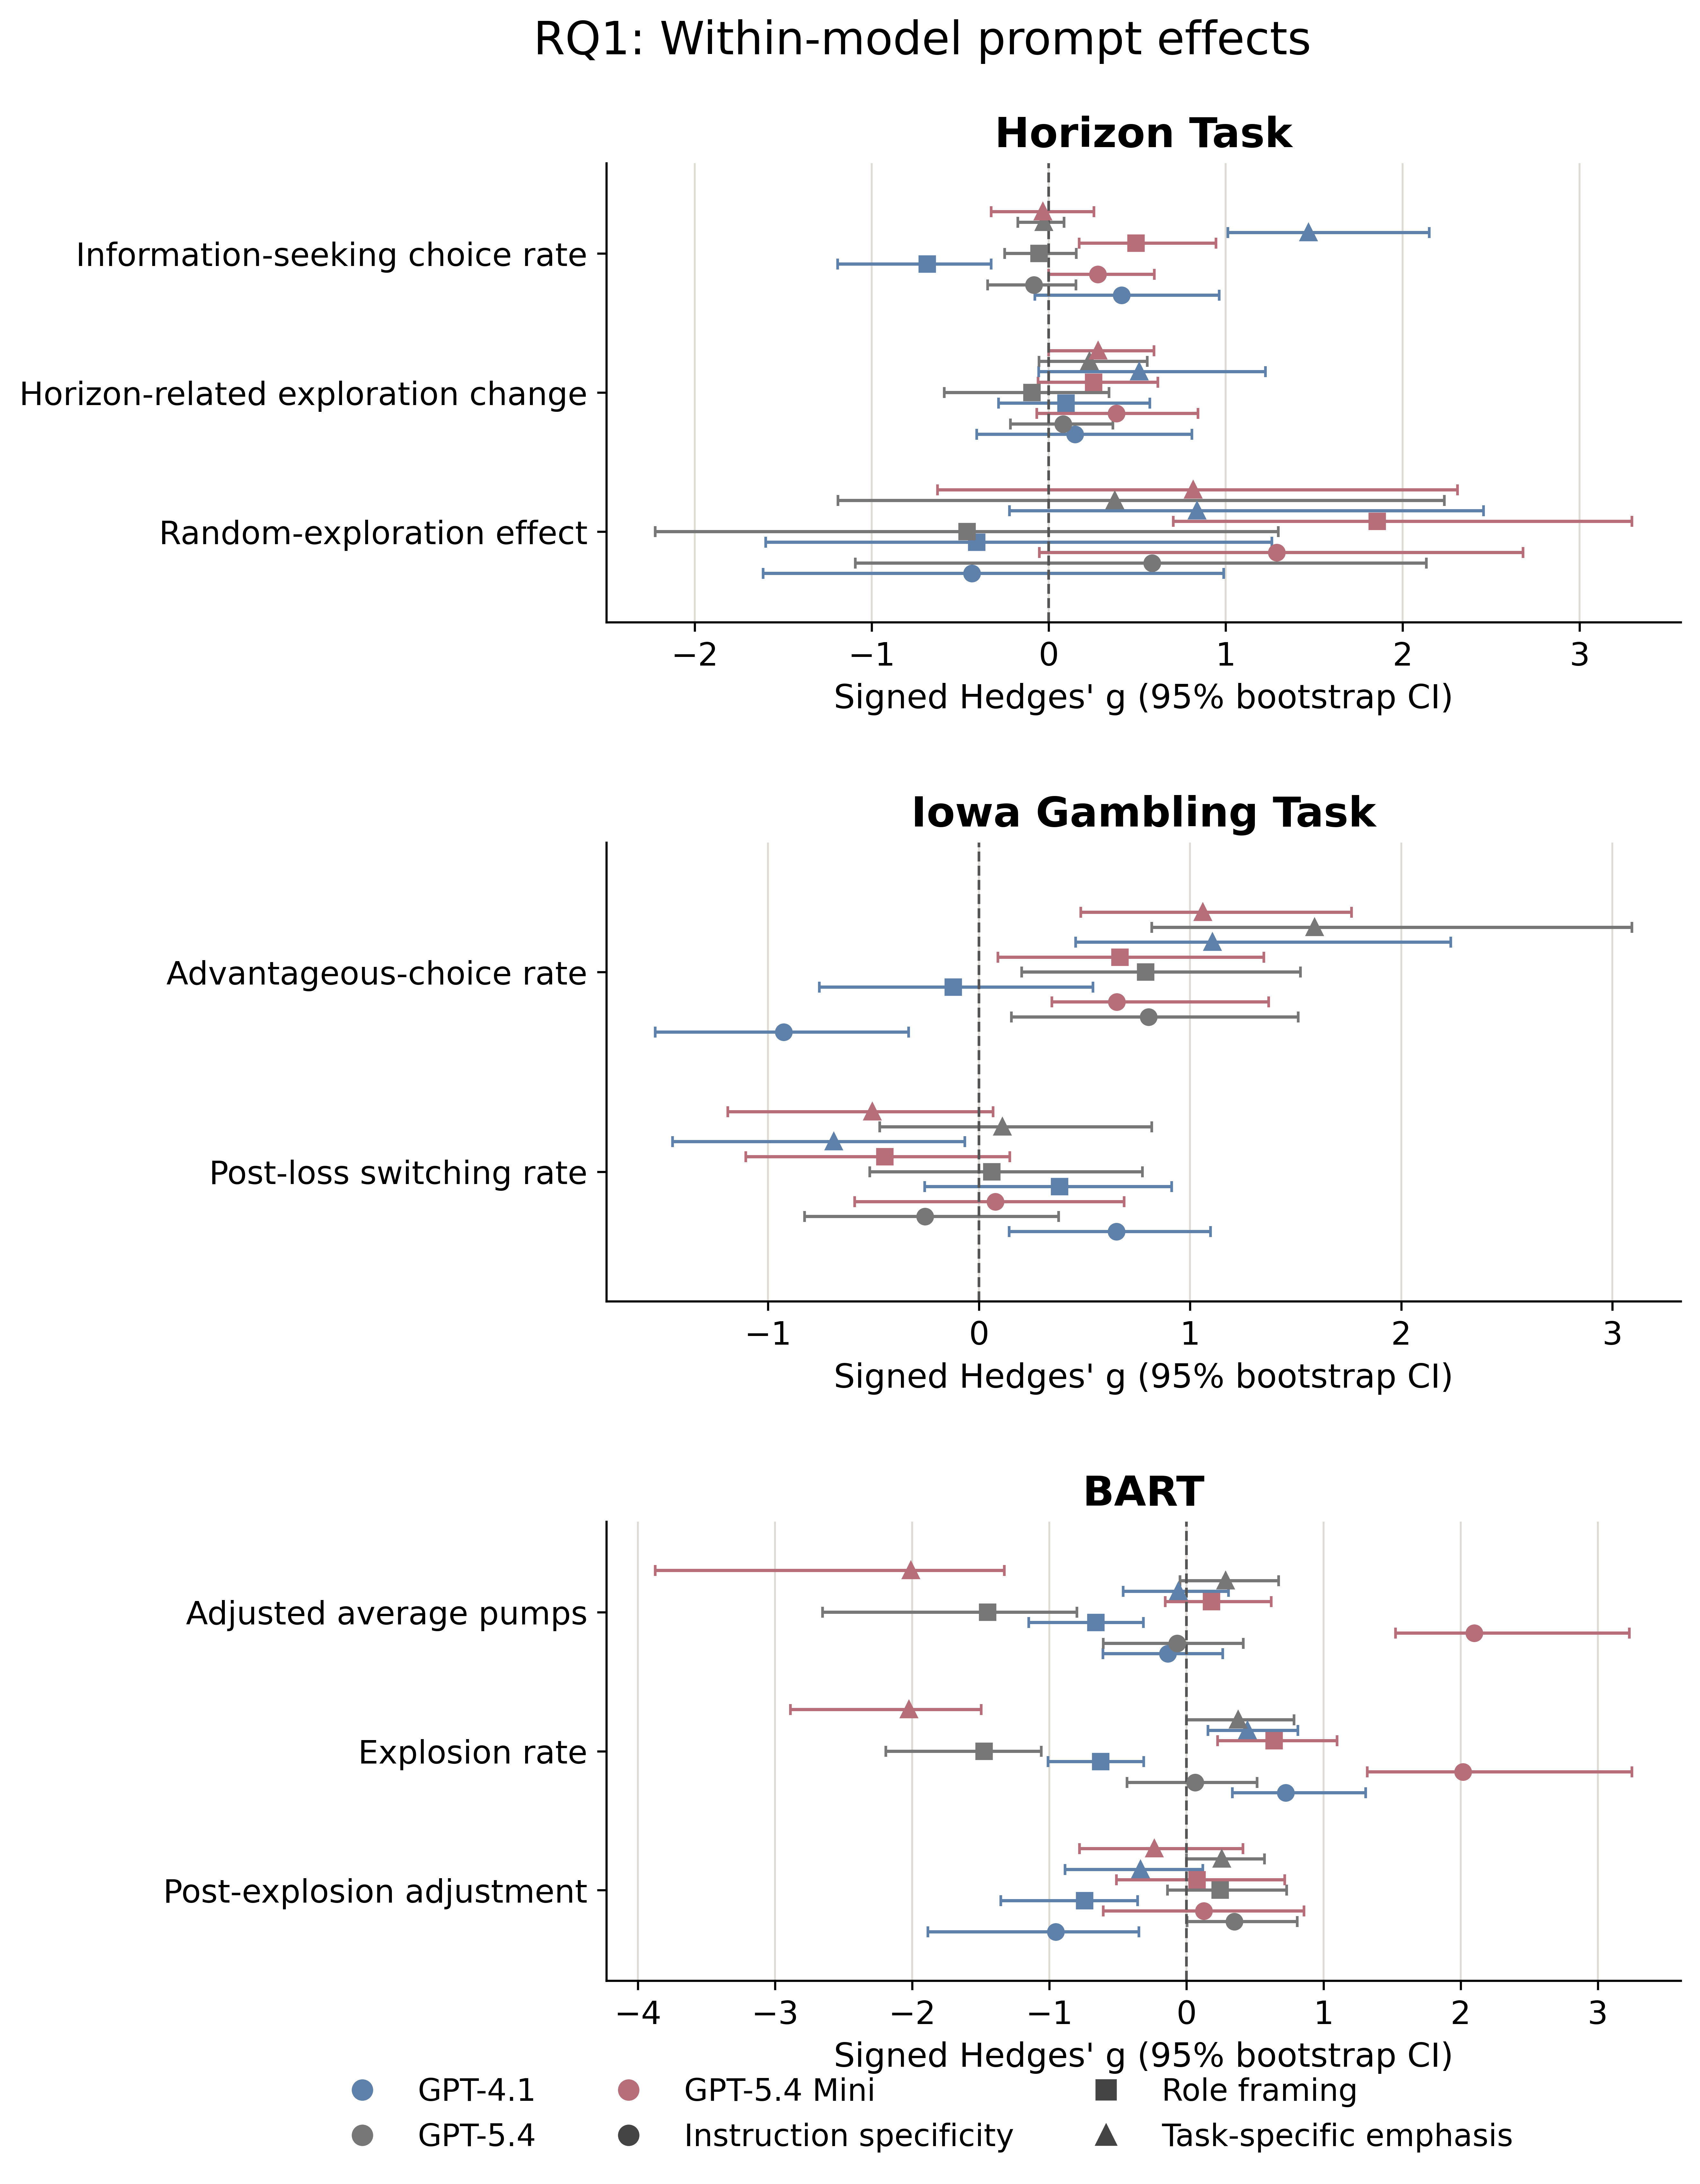
\includegraphics[width=0.96\textwidth,height=0.80\textheight,keepaspectratio]{figure_rq1_prompt_effects_overview.png}
\caption{Within-model prompt effects relative to Neutral. Points show signed Hedges' $g$; lines show 95\% bootstrap confidence intervals.}
\label{fig:rq1}
\end{figure}

\section{RQ2: Cross-Model Variation in Prompt Effects}
Figure~\ref{fig:rq2} reports $(\text{candidate condition}-\text{candidate Neutral})-(\text{GPT-5.4 condition}-\text{GPT-5.4 Neutral})$; positive values therefore indicate a more positive prompt response in the candidate model. The contrasts were concentrated in particular outcomes rather than showing a common amplification or attenuation across all prompt effects. Of the 48 interaction contrasts (two candidate models, three conditions, and eight metrics), 19 intervals excluded zero and 29 straddled it, confirming that reliable cross-model differences were localised rather than pervasive. Differences between GPT-4.1 and GPT-5.4 were most visible in Horizon information seeking, IGT advantageous choices, and BART post-explosion adjustment. For the latter outcome, the instruction-specificity interaction was -1.7361 pumps ([-2.6121, -0.8463]).

Mini differed most clearly from GPT-5.4 in BART. Its adjusted-pump interaction was 2.0260 ([1.4853, 2.5801]) for instruction specificity but -1.5486 ([-1.8790, -1.1836]) for risk emphasis, accompanied by changes in the direction of explosion-rate effects. In Horizon, the Role-framing Random-exploration interaction was 2.1337 ([0.7465, 3.6430]). Thus, the cross-model evidence identifies differences in response to the same formulation manipulation; it does not rank general model capability and cannot be inferred from baseline differences alone.

\begin{figure}[!tbp]
\centering
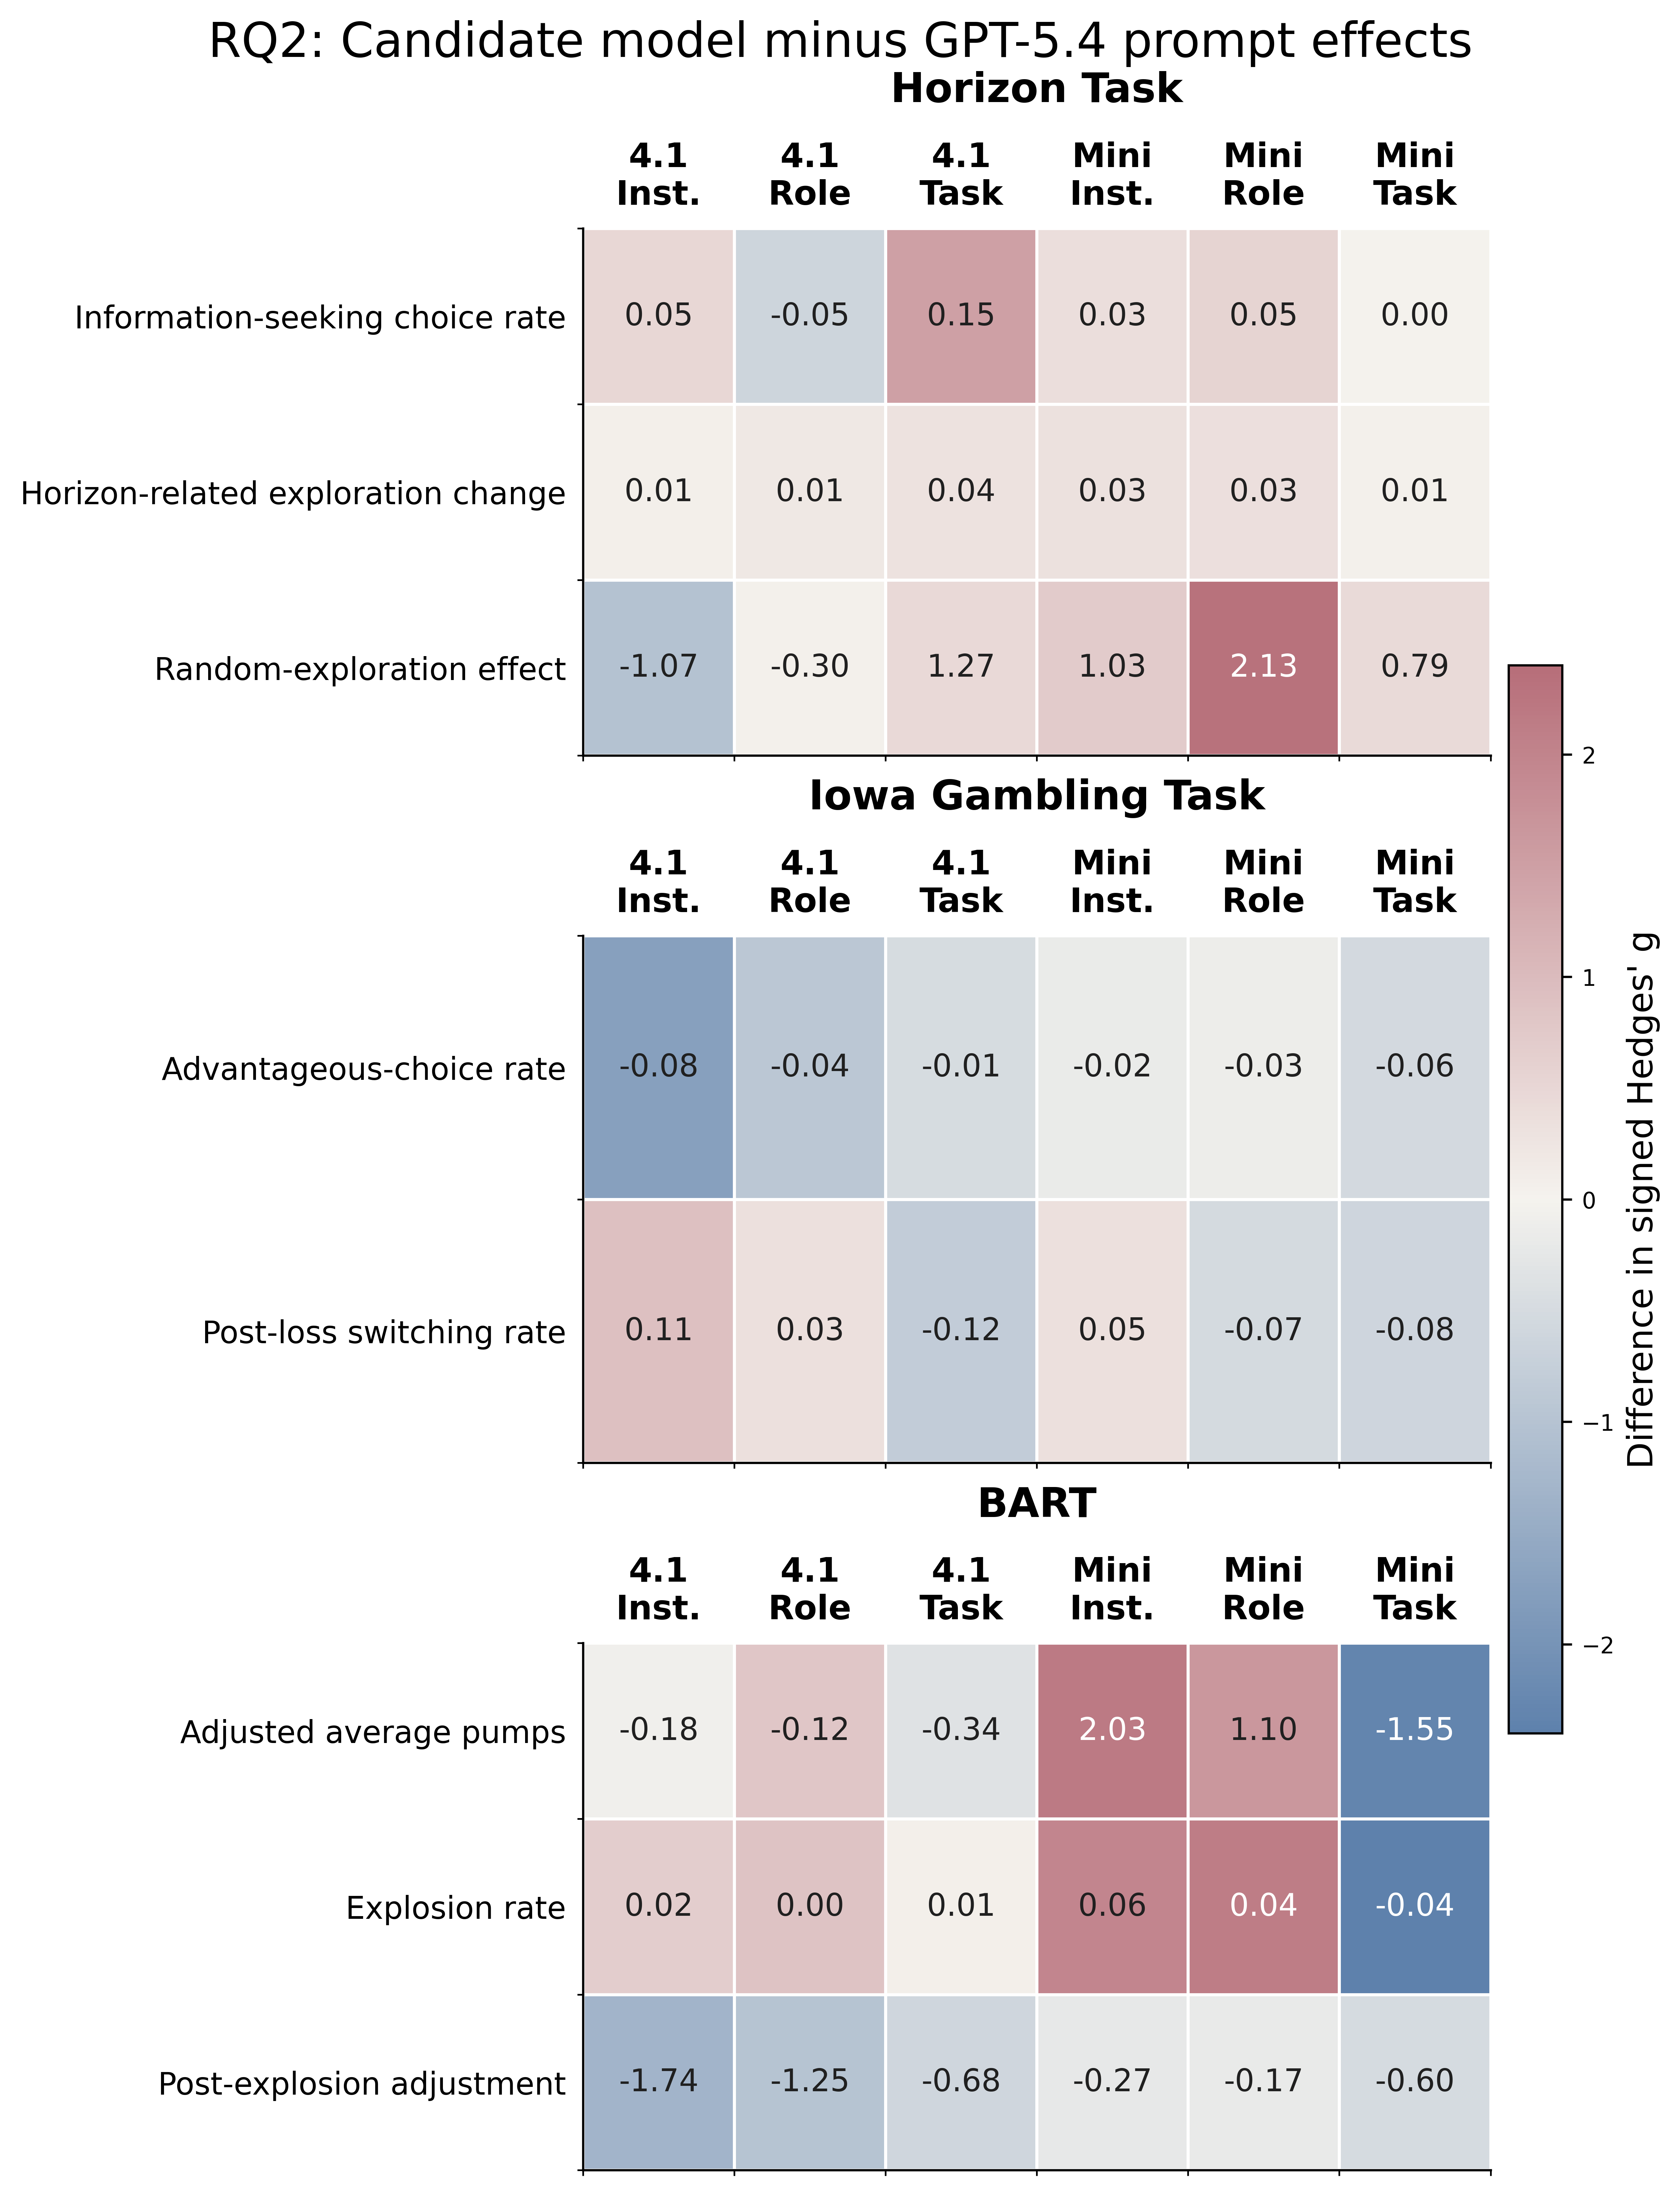
\includegraphics[width=0.96\textwidth,height=0.80\textheight,keepaspectratio]{figure_rq2_model_interactions_overview.png}
\caption{Model-by-prompt interactions relative to GPT-5.4. Cell text gives raw contrasts; colour shows differences in signed Hedges' $g$.}
\label{fig:rq2}
\end{figure}

\section{RQ3: Cross-Language Variation}
Figure~\ref{fig:rq3} assigns the three languages equal status. Panel A shows pooled-SD-scaled centred Neutral baselines and Panel B shows each language's Hedges' $g$ relative to the three-language mean $g$; the examples below instead use raw metric units. Across the 24 centred baselines, 15 intervals excluded zero, and across the 72 centred prompt effects, 31 did, so language-associated differences appeared in both baseline location and prompt response but not uniformly across tasks and metrics. Horizon information-seeking baseline deviations were -0.0267 (95\% CI [-0.0533, -0.0008]) for English, -0.0467 ([-0.0675, -0.0300]) for Simplified Chinese, and 0.0733 ([0.0500, 0.0958]) for Spanish. For IGT post-loss switching, the corresponding deviations were 0.0781, -0.2000, and 0.1219. These profiles show that language-associated variation was already present under Neutral prompts.

Within-language prompt responses also occupied different centred positions. For Horizon uncertainty emphasis and information seeking, the deviations were 0.0908 ([0.0600, 0.1225]) in English, -0.0067 ([-0.0300, 0.0183]) in Chinese, and -0.0842 ([-0.1067, -0.0600]) in Spanish. For IGT reward--loss emphasis and advantageous choices, they were 0.0593, -0.0617, and 0.0023; Spanish BART instruction specificity deviated by 0.9073 adjusted pumps ([0.4254, 1.4286]). Each triplet sums to zero by construction. RQ3 therefore distinguishes centred baseline location from centred prompt-response variation without treating any language as the reference.

\begin{figure}[!tbp]
\centering
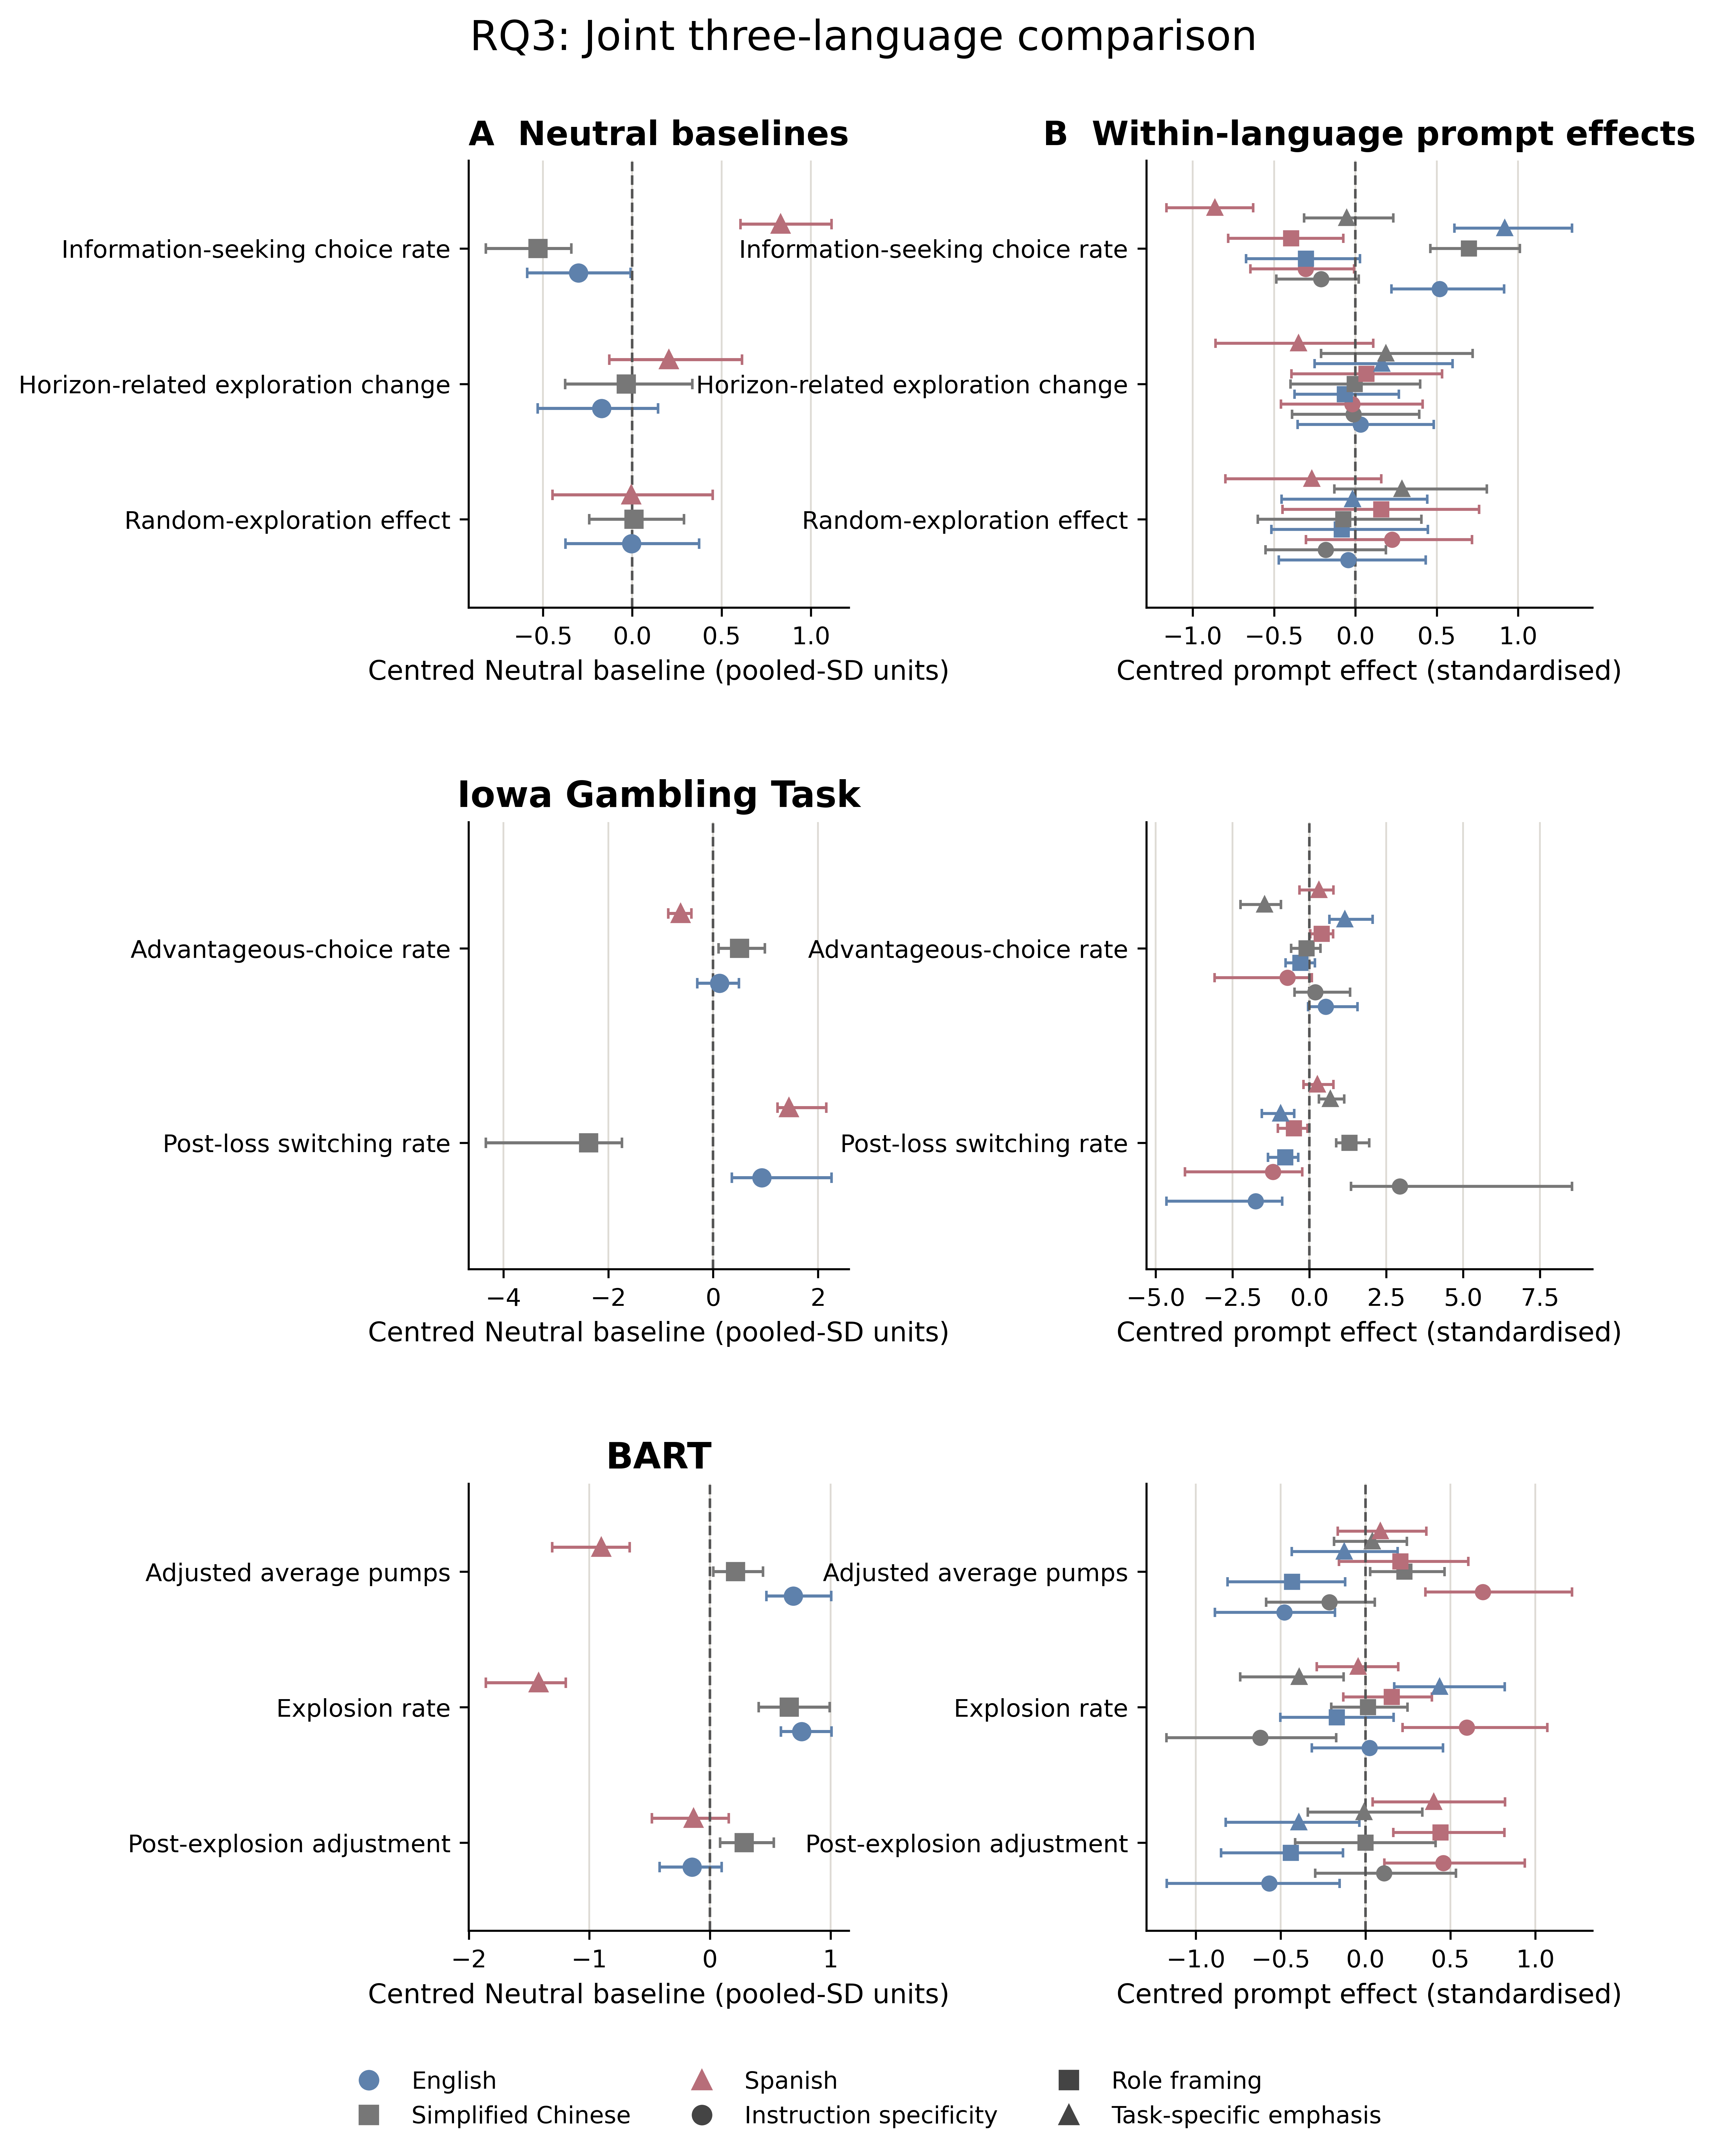
\includegraphics[width=0.96\textwidth,height=0.72\textheight,keepaspectratio]{figure_rq3_language_overview.png}
\caption{Joint centred three-language comparison. Panel A: standardised Neutral baselines; Panel B: centred prompt effects. No language is the reference.}
\label{fig:rq3}
\end{figure}

\section{RQ4: Prompt-Associated Proximity Changes}
Figure~\ref{fig:rq4} contains descriptive point estimates. Run-level bootstrap 95\% intervals (2,000 replicates, seed 20260615, human reference held fixed) were additionally constructed for the seven directly computed metrics; the hierarchical random-exploration metric is excluded because its human-side estimate is model-based rather than a participant-level summary. Negative absolute-deviation change denotes movement of the cell mean towards the human mean, whereas positive coverage change denotes greater overlap between run-level values and the empirical human range. Coverage uses the non-missing runs in each cell, giving a resolution of 0.05 when all 20 runs are available. Neither direction is a test of distributional equivalence or shared cognitive mechanism.

No formulation improved both proximity measures uniformly. English GPT-4.1 Horizon uncertainty emphasis increased absolute information-seeking deviation by 1.711 human-SD units (95\% bootstrap interval $[0.866, 2.144]$) and reduced coverage by 0.40 ($[-0.65, -0.10]$). Chinese GPT-4.1 IGT instruction specificity reduced the post-loss-switching deviation by 1.428 ($[-1.550, -1.250]$) while leaving coverage unchanged ($[0.00, 0.00]$). Mini BART instruction specificity reduced adjusted-pump deviation by 0.602 ($[-0.729, -0.477]$) and increased coverage by 0.85 ($[0.70, 1.00]$). Across the 120 cells, absolute mean deviation moved closer to the human mean in 69, farther in 50, and was unchanged in one; coverage changed in 65 cells and was unchanged in the remaining 55, with the two measures moving in opposite directions in 49 cells. The reference means themselves carried modest sampling uncertainty: bootstrap 95\% intervals for the reference mean had half-widths from 0.014 to 0.556 in the original metric units across the seven directly computed metrics (for example, Horizon information seeking 0.524--0.564, IGT advantageous choices 0.525--0.552, and BART adjusted pumps 7.761--8.873). The mixture of positive, negative, and near-zero cells confirms that mean location and run-level overlap can change separately; classifications such as ``closer'' refer only to the direction of the absolute-deviation point estimate, and neither measure can stand in for the other.

\begin{figure}[!tbp]
\centering
\includegraphics[width=1.0\textwidth,height=0.80\textheight,keepaspectratio]{figure_rq4_human_reference_overview.png}
\caption{Prompt-associated changes in absolute mean deviation (left) and empirical coverage (right) relative to Neutral.}
\label{fig:rq4}
\end{figure}


\FloatBarrier
\chapter{Discussion}
\label{sec:discussion}

\section{Integrated Findings and Methodological Contribution}

The results reveal conditionality at three distinct levels rather than one generic ``prompt effect''. First, formulation changed behaviour within a fixed model: for GPT-4.1, Horizon Role framing reduced information seeking by 0.0575 whereas uncertainty emphasis increased it by 0.1450. Second, the same manipulation did not transfer predictably between models: Mini's BART adjusted pumps increased by 1.9763 under instruction specificity but decreased by 1.3114 under risk emphasis, while the corresponding interactions relative to GPT-5.4 were 2.0260 and -1.5486. Third, even a fixed model and formulation did not transfer straightforwardly between language implementations: the centred Horizon uncertainty-emphasis effect was positive in English (0.0908), near zero in Chinese (-0.0067), and negative in Spanish (-0.0842). The substantive conclusion is therefore stronger than saying that wording ``matters'': the sign of an apparent exploration or risk-taking effect can depend on the model--prompt--language measurement configuration.

This pattern also explains why a single cross-task reliability score would be misleading. The instability was concentrated in particular model--outcome combinations rather than uniformly distributed. GPT-5.4's Horizon effects were comparatively small, yet its IGT advantageous-choice rate increased under all three manipulations; Mini showed especially large and oppositely directed BART changes. Aggregating these results could cancel meaningful reversals or allow one volatile metric to dominate. The evaluation framework consequently treats the raw, task-specific contrast as the estimand and uses standardised plots and PSI only to locate sensitivity. Its methodological contribution is not a new claim that one model is globally more reliable, but a procedure for determining exactly which conclusion survives controlled changes to the measurement instrument.

\section{Conditionality of LLM Behavioural Measurement}

The direction reversals help distinguish two interpretations of prompt sensitivity. If formulations merely added unsystematic sampling noise, effects should fluctuate around zero without reproducible structure. Instead, construct emphasis produced directional changes in some cells, and matched manipulations generated sharply different responses across models. This extends prior multi-template evidence from mostly static evaluations \cite{Sclar2024PromptFormatting,Mizrahi2024MultiPrompt} by showing structured formulation dependence in summaries of complete sequential runs. A plausible measurement interpretation is that prompts alter the salience of candidate policies: uncertainty language can make information acquisition more locally relevant, while risk language can make stopping or cashing out more salient. The GPT-4.1 Horizon increase under uncertainty emphasis and Mini BART decrease under risk emphasis are consistent with this account. However, this remains a behavioural explanation, not evidence that the models possess the named human constructs; the Role-framing reversal and weak GPT-5.4 Horizon effects show that cue uptake is mediated by the model and task context.

RQ2 further shows why baseline performance cannot diagnose robustness. A model can occupy a similar Neutral baseline yet react differently once a cue is introduced; the estimand is the difference in changes, not the difference in starting levels. The Mini--GPT-5.4 BART interactions demonstrate this particularly clearly: instruction specificity and risk emphasis moved the interaction in opposite directions within the same task and metric. Robustness is therefore a property of a model's response surface over plausible measurement formulations, rather than a property that can be inferred from one benchmark score or one Neutral run. This result sharpens earlier reports of model-dependent prompt sensitivity \cite{Zhuo2024ProSA} and reinforces the need to bind conclusions to recorded proprietary snapshots and collection dates \cite{Chen2024ChatGPTBehavior,Palmer2024ProprietaryModels}.

RQ3 adds a second layer to this response surface. Spanish had a higher centred Neutral location for Horizon information seeking (0.0733), but its centred response to uncertainty emphasis was negative. Baseline language differences therefore did not predict prompt-effect differences. This rules out a simple account in which one language implementation merely shifts all responses by a constant amount. It also extends benchmark evidence of cross-language inconsistency \cite{Qi2023CrossLingualConsistency} to both Neutral locations and within-language prompt responses in sequential tasks. Because translation also changes wording length, information order, pragmatic force, and salience, and because Chinese and Spanish were collected later, these are language-associated measurement differences rather than isolated causal effects of language. Practically, translating a validated English prompt does not preserve a behavioural instrument automatically; both the Neutral baseline and each manipulation require revalidation.

Finally, the task metrics show why direction must be interpreted locally. More Horizon information seeking may reflect directed exploration, but more BART pumps simultaneously increase potential reward and explosion exposure; IGT advantageous choice and post-loss switching capture different aspects of feedback use. The absence of coordinated movement between IGT metrics and the reversals among BART outcomes mean that ``more'' cannot be equated with better reasoning, greater rationality, or greater human-likeness. The meaningful unit of interpretation is a named behavioural outcome under a specified task implementation.

\section{Human Reference and Interpretive Boundaries}

RQ4 makes the consequences of this conditionality concrete. Mini's BART instruction-specificity condition moved its adjusted-pump mean 0.602 human SDs closer to the human mean and increased empirical coverage by 0.85, so both location and overlap changed in the same direction. In contrast, Chinese IGT instruction specificity reduced the post-loss-switching deviation by 1.428 but left coverage unchanged. English GPT-4.1 Horizon uncertainty emphasis moved the mean 1.711 human SDs farther away and reduced coverage by 0.40. These cases show that a prompt can change the centre of the generated runs without changing how broadly they occupy the human empirical interval, or can change both.

The two measures answer different questions. Absolute mean deviation asks where the LLM cell centre lies relative to the human mean; empirical coverage asks what fraction of LLM runs falls inside a fixed human range. A concentrated distribution can have a close mean but low coverage, while a dispersed distribution can achieve high coverage despite a displaced mean. With 20 runs, coverage also changes in increments of 0.05, making small differences intrinsically coarse. It follows that selecting a prompt because it improves only one proximity measure would embed an unacknowledged choice about what ``human-like'' means.

More fundamentally, neither measure identifies a shared cognitive mechanism or a human population distribution. The repeated runs share a model snapshot, deployment, prompt, and task implementation; they estimate stochastic variation under that system, not independent persons with stable individual histories. This boundary is consistent with critiques of treating synthetic responses as interchangeable participants \cite{Dillion2023ReplaceParticipants,Bisbee2024SyntheticSurveyData}. Human-reference proximity should therefore be used as a diagnostic coordinate for comparing measurement specifications, not as validation that an LLM can replace participants or instantiate the same latent process. Nor is proximity a normative standard: the study does not claim that an LLM should behave like humans to be a good cognitive model, and the human reference fixes a coordinate system for comparing measurement specifications rather than a target for model quality.

\section{Limitations, Reproducibility Implications, and Future Work}

The design establishes that conditionality exists within the tested configuration, but it cannot fully decompose its causes. Twenty runs per cell provide complete balanced comparisons yet give limited information about rare policies, distributional tails, and high-variance interactions; bootstrap intervals quantify the information in those runs but cannot manufacture additional independent variation. The particularly large BART interactions should therefore motivate higher-powered replication rather than claims that BART is intrinsically more prompt-sensitive. Likewise, the shrinkage sensitivity of Random exploration means that conclusions about that latent parameter remain partly dependent on the fitted hierarchical model, even though all formal fits converged.

The prompt variants were information-matched, not feature-orthogonal. Semantic emphasis co-varied with length, repetition, position, and lexical salience, so the experiment estimates the effect of each complete formulation rather than the isolated causal effect of ``role'', ``specificity'', or ``risk''. Multilingual informational review did not establish cultural or pragmatic equivalence, and the later Chinese and Spanish collection leaves language implementation partially confounded with temporal drift. The human comparisons add further asymmetry: task length, familiarisation, and presentation differed between LLM and human sources, while reference-summary uncertainty was quantified by bootstrap but not propagated through the cell-level deviation and coverage changes; run-level resampling intervals are reported for the seven directly computed metrics, so the RQ4 point estimates carry sampling uncertainty without assuming a precise human population benchmark. These boundaries narrow the claim to measurement robustness; they do not weaken the observed fact that reported behavioural conclusions changed under plausible implementations.

Future work should proceed in the order implied by the results. First, the largest sign reversals should be replicated with larger cells and independent collection dates to distinguish persistent response structure from snapshot-specific behaviour. Second, factorial prompt designs should manipulate semantic emphasis, length, position, and keyword salience separately. Third, translations should be independently validated and collected concurrently, with equivalence assessed behaviourally rather than assumed from informational matching. Finally, human-reference analyses should propagate reference-sample uncertainty through the cell-level deviation and coverage changes and compare fuller distributional features under better-aligned task implementations. Across these extensions, prompts, model versions, failures, repairs, dates, and resampling diagnostics must remain part of the reported measurement specification.

The framework itself is not tied to the three tasks or to text-only models. Its components---a fixed measurement specification, prespecified formulation variants, complete trajectories as the replication unit, bootstrap uncertainty, and a descriptive reference comparison---apply to any system whose behaviour can be sampled repeatedly, including vision-language models, tool-using agents, and embodied decision-makers. A minimal transfer checklist would therefore need to freeze the new degrees of freedom introduced by perception, tool calls, and environment interfaces; specify the formulation-variant space in the new modality (for example, visual-context, instruction, and tool-policy variants); extend the response-parsing specification to the system's action vocabulary; and keep trajectories, seeds, snapshots, failures, and resampling diagnostics inside the reported measurement specification. The analytic logic---condition-minus-baseline contrasts, model-by-prompt interactions, and a descriptive reference comparison---would remain unchanged.

Taken together, the evidence does not support a prompt ranking that remains constant across conditions. It supports a narrower, auditable conclusion: LLM results in decision-making tasks show systematic but task-specific sensitivity to the measurement specification. Reliable use of such evidence requires joint reporting of the formulation, model snapshot, language, behavioural outcome, and uncertainty, while retaining human-reference proximity as a conditional descriptive comparison.

\chapter{Conclusions}
\label{sec:conclusion}

How reliable, then, are LLMs as cognitive models? Under the behavioural definition adopted in this dissertation, the answer is conditional. The tested systems cannot be regarded as reliably prompt-invariant models of cognition: observed effects varied across model snapshots, tasks, outcomes, and language implementations, and the same prompt manipulation could produce changes in opposite directions across models or outcomes. They can nevertheless serve as useful computational models of cognitive-task behaviour when claims are restricted to an explicit measurement specification and their robustness is evaluated across prespecified formulations. Prompt sensitivity was structured and conditional, rather than a general effect captured by a single ranking of formulations; claims about exploration, response to feedback, or risk taking should therefore not be generalised directly from one prompt, model snapshot, or language implementation.

The study's principal contribution is an auditable evaluation framework for locating this conditionality. It treats a complete task run as the unit of repeated generation, compares prespecified prompt variants with matched informational boundaries, directly estimates cross-model interaction contrasts and three-language centred deviations, and distinguishes task-specific behaviour, prompt sensitivity, and human-reference proximity. The human-reference analyses further show that the proximity of a cell mean to the human mean and the overlap of run-level values with an empirical human range can change separately across prompts. Both are descriptive references: neither demonstrates a shared cognitive mechanism nor establishes distributional equivalence between LLM runs and the human participant population.

Future work should prioritise replication at different collection times and across additional model snapshots, together with larger numbers of runs per cell to improve the precision of estimates for variable outcomes, rare strategies, and interaction effects. Orthogonal designs could then separate the contributions of semantic emphasis, prompt length, information position, and keyword salience. Multilingual research would benefit from independent translation validation and more closely synchronised data collection to reduce confounding between translation implementation and temporal drift. Human-reference analyses should propagate reference-sample uncertainty through cell-level proximity changes and more closely align task length, information presentation, and measurement precision. By releasing prompts, model and collection-version information, the full analysis workflow, parser repairs, and data-quality records, future studies can more reliably distinguish behavioural regularities that persist across measurement implementations from findings produced by a particular experimental configuration.
% \section{Final Reminder}

% The body of your dissertation, before the references and any appendices,
% \emph{must} finish by page~40. The introduction, after preliminary material,
% should have started on page~1.

% You may not change the dissertation format (e.g., reduce the font size, change
% the margins, or reduce the line spacing from the default 1.5 spacing). Be
% careful if you copy-paste packages into your document preamble from elsewhere.
% Some \LaTeX{} packages, such as \texttt{fullpage} or \texttt{savetrees}, change
% the margins of your document. Do not include them!

% Over-length or incorrectly-formatted dissertations will not be accepted and you
% would have to modify your dissertation and resubmit. You cannot assume we will
% check your submission before the final deadline and if it requires resubmission
% after the deadline to conform to the page and style requirements you will be
% subject to the usual late penalties based on your final submission time.

\bibliographystyle{unsrt}
\bibliography{mybibfile}


\appendix
\sloppy

\chapter{Research Materials and Supplementary Results}
\label{app:materials}

This appendix identifies the materials supporting reproduction and audit of the
study. The complete files are deposited in the online research repository cited
in the Reproducibility section. The links below refer to that repository rather
than to the local or Overleaf project filesystem. The 36 frozen prompt files are
reproduced verbatim in Appendix~\ref{app:prompts}, and the terminology mapping
between dissertation terms, code identifiers, and the three prompt languages is
given in Appendix~\ref{app:terminology}. Complete cell-level outputs are indexed
rather than reproduced, because they would add substantial length without adding
evidence required to follow the main argument.

\section{Frozen Prompt Materials}

For each task, the four formal conditions were Neutral, Instruction
specificity, Role framing, and Task-specific construct emphasis. The frozen
English files follow the naming scheme \texttt{baseline.md} (Neutral),
\texttt{detailed.md} (Instruction specificity), \texttt{role\_human.md} (Role
framing), and \texttt{uncertainty\_emphasis.md},
\texttt{reward\_loss\_emphasis.md}, and \texttt{risk\_emphasis.md}
(Task-specific construct emphasis) under \url{prompts/TASK/}, where
\texttt{TASK} is \texttt{bandit}, \texttt{igt}, or \texttt{bart}. The
Simplified Chinese and Spanish versions of all four conditions are under
\url{prompts/multilingual/zh-CN/TASK/} and
\url{prompts/multilingual/es/TASK/}.

The complete prompt collection is available in the \url{prompts/} directory of
the research repository linked in the Reproducibility section. The
prompt-development protocol and provenance are in \url{prompts/generation/},
including the dated generation records.
Multilingual constraints and the completed audit trail are in
\url{prompts/multilingual/}. These records document informational checks and
freezing; they do not establish complete pragmatic or cultural equivalence.

\section{Verbatim Prompt Texts}
\label{app:prompts}

The 36 frozen prompt files are reproduced below as used in data collection. Line breaks are reflowed for readability; paragraph boundaries, fenced response-format blocks, and placeholder tokens are preserved. English texts are followed by Simplified Chinese and Spanish; within each language the order is Horizon Task, Iowa Gambling Task, and BART, with the four conditions per task. Placeholders such as \texttt{\{observation\}} are literal template tokens from the frozen files; the runner substituted the current task state at every decision.

\subsection*{English --- Horizon Task --- Neutral}
\begin{quote}\ttfamily\footnotesize
\# Two-Option Reward Task \\
\\
You will complete 40 separate games. In each game, you make a \\
series of choices between option A and option B. \\
\\
Each game begins with four forced choices. On a forced-choice \\
trial, the current task state tells you which option you must \\
choose. After these four choices, you will make either one or six \\
free choices between A and B. \\
\\
Within a game, A and B may have different reward patterns that are \\
not known to you in advance. After every choice, you are shown the \\
reward from the selected option. You may use the observed rewards \\
and the number of choices remaining in the current game when \\
making later choices. \\
\\
Your aim is to finish the full task with as much total reward as \\
possible. \\
\\
Current task state: \\
\\
```text \\
\{observation\} \\
``` \\
\\
Valid responses: \\
\\
```text \\
CHOICE: A \\
CHOICE: B \\
``` \\
\\
Respond with exactly one valid response and no additional text. \\
\end{quote}


\subsection*{English --- Horizon Task --- Instruction specificity}
\begin{quote}\ttfamily\footnotesize
\# Two-Option Reward Task \\
\\
You will complete 40 separate games. Each game consists of a \\
series of choices between two options: \\
option A and option B. \\
\\
At the start of each game, you will make four forced choices. \\
During these forced-choice trials, the current task state will \\
specify which option you must select. After completing these four \\
forced choices, you will proceed to make either one or six free \\
choices, where you can freely choose between option A and option \\
B. \\
\\
Within each game, the reward patterns for options A and B may \\
differ, and these patterns are not revealed to you beforehand. \\
After every choice you make, you will receive feedback showing the \\
reward associated with the option you selected. You can use the \\
rewards you observe, along with the number of remaining choices in \\
the current game, to inform your subsequent decisions. \\
\\
Your aim is to finish the full task with as much total reward as \\
possible. \\
\\
Current task state: \\
\\
```text \\
\{observation\} \\
``` \\
\\
Valid responses: \\
\\
```text \\
CHOICE: A \\
CHOICE: B \\
``` \\
\\
Respond with exactly one valid response and no additional text. \\
\end{quote}


\subsection*{English --- Horizon Task --- Role framing}
\begin{quote}\ttfamily\footnotesize
\# Two-Option Reward Task \\
\\
Take the role of a human participant completing this task. \\
\\
You will complete 40 separate games. In each game, you make a \\
series of choices between option A and option B. \\
\\
Each game begins with four forced choices. On a forced-choice \\
trial, the current task state tells you which option you must \\
choose. After these four choices, you will make either one or six \\
free choices between A and B. \\
\\
Within a game, A and B may have different reward patterns that are \\
not known to you in advance. After every choice, you are shown the \\
reward from the selected option. You may use the observed rewards \\
and the number of choices remaining in the current game when \\
making later choices. \\
\\
Your aim is to finish the full task with as much total reward as \\
possible. \\
\\
Current task state: \\
\\
```text \\
\{observation\} \\
``` \\
\\
Valid responses: \\
\\
```text \\
CHOICE: A \\
CHOICE: B \\
``` \\
\\
Respond with exactly one valid response and no additional text. \\
\end{quote}


\subsection*{English --- Horizon Task --- Construct emphasis (uncertainty)}
\begin{quote}\ttfamily\footnotesize
\# Two-Option Reward Task \\
\\
You will complete 40 separate games. In each game, you make a \\
series of choices between option A and option B. \\
\\
Each game begins with four forced choices. On a forced-choice \\
trial, the current task state tells you which option you must \\
choose. After these four choices, you will make either one or six \\
free choices between A and B. \\
\\
Within a game, A and B may have different reward patterns that are \\
not known to you in advance. Each observed reward provides only \\
partial information about those patterns. After every choice, you \\
are shown the reward from the selected option. You may use this \\
incomplete information and the number of choices remaining in the \\
current game when making later choices. \\
\\
Your aim is to finish the full task with as much total reward as \\
possible. \\
\\
Current task state: \\
\\
```text \\
\{observation\} \\
``` \\
\\
Valid responses: \\
\\
```text \\
CHOICE: A \\
CHOICE: B \\
``` \\
\\
Respond with exactly one valid response and no additional text. \\
\end{quote}


\subsection*{English --- Iowa Gambling Task --- Neutral}
\begin{quote}\ttfamily\footnotesize
\# Four-Deck Reward Task \\
\\
You will make 100 choices. Your cumulative score starts at 2000. \\
\\
On each trial, choose one of four decks: \\
A, B, C, or D. Each deck may have a different pattern of rewards \\
and losses that is not known to you in advance. After every \\
choice, you are shown the reward, any loss, the net outcome, and \\
your updated cumulative score. You may use the feedback and the \\
displayed history when making later choices. \\
\\
Your aim is to finish the full task with as much total reward as \\
possible. \\
\\
Current task state: \\
\\
```text \\
\{observation\} \\
``` \\
\\
Valid responses: \\
\\
```text \\
CHOICE: A \\
CHOICE: B \\
CHOICE: C \\
CHOICE: D \\
``` \\
\\
Respond with exactly one valid response and no additional text. \\
\end{quote}


\subsection*{English --- Iowa Gambling Task --- Instruction specificity}
\begin{quote}\ttfamily\footnotesize
\# Four-Deck Reward Task \\
\\
You will make a total of 100 choices during this task. Your \\
cumulative score begins at 2000 points. \\
\\
On each trial, you will select one of four decks: \\
A, B, C, or D. Each deck may have a different pattern of rewards \\
and losses, but these patterns are not known to you at the start \\
of the task. After making a choice, you will receive feedback that \\
includes: \\
\\
- The reward you received from the chosen deck. - Any loss \\
associated with the chosen deck. - The net outcome. - Your updated \\
cumulative score. \\
\\
You can use the feedback provided after each choice, as well as \\
the displayed history of your previous choices and outcomes, to \\
inform your decisions in subsequent trials. \\
\\
Your aim is to finish the full task with as much total reward as \\
possible. \\
\\
Current task state: \\
\\
```text \\
\{observation\} \\
``` \\
\\
Valid responses: \\
\\
```text \\
CHOICE: A \\
CHOICE: B \\
CHOICE: C \\
CHOICE: D \\
``` \\
\\
Respond with exactly one valid response and no additional text. \\
\end{quote}


\subsection*{English --- Iowa Gambling Task --- Role framing}
\begin{quote}\ttfamily\footnotesize
\# Four-Deck Reward Task \\
\\
Take the role of a human participant completing this task. \\
\\
You will make 100 choices. Your cumulative score starts at 2000. \\
\\
On each trial, choose one of four decks: \\
A, B, C, or D. Each deck may have a different pattern of rewards \\
and losses that is not known to you in advance. After every \\
choice, you are shown the reward, any loss, the net outcome, and \\
your updated cumulative score. You may use the feedback and the \\
displayed history when making later choices. \\
\\
Your aim is to finish the full task with as much total reward as \\
possible. \\
\\
Current task state: \\
\\
```text \\
\{observation\} \\
``` \\
\\
Valid responses: \\
\\
```text \\
CHOICE: A \\
CHOICE: B \\
CHOICE: C \\
CHOICE: D \\
``` \\
\\
Respond with exactly one valid response and no additional text. \\
\end{quote}


\subsection*{English --- Iowa Gambling Task --- Construct emphasis (reward/loss)}
\begin{quote}\ttfamily\footnotesize
\# Four-Deck Reward Task \\
\\
You will make 100 choices. Your cumulative score starts at 2000. \\
\\
On each trial, choose one of four decks: \\
A, B, C, or D. Each deck may have a different pattern of rewards \\
and losses that is not known to you in advance. After every \\
choice, pay particular attention to the reward, any loss, the net \\
outcome, and your updated cumulative score. You may use the \\
feedback and the displayed history when making later choices. \\
\\
Your aim is to finish the full task with as much total reward as \\
possible. \\
\\
Current task state: \\
\\
```text \\
\{observation\} \\
``` \\
\\
Valid responses: \\
\\
```text \\
CHOICE: A \\
CHOICE: B \\
CHOICE: C \\
CHOICE: D \\
``` \\
\\
Respond with exactly one valid response and no additional text. \\
\end{quote}


\subsection*{English --- Balloon Analogue Risk Task --- Neutral}
\begin{quote}\ttfamily\footnotesize
\# Balloon Earnings Task \\
\\
You will complete 40 balloons. For each balloon, choose either to \\
pump the balloon or to cash out. \\
\\
Every successful pump adds 0.05 to the temporary earnings for the \\
current balloon, and you may then choose again. A pump can also \\
cause the balloon to explode. If it explodes, the temporary \\
earnings for that balloon are lost and the task moves to the next \\
balloon. \\
\\
If you cash out, the current temporary earnings are added to your \\
total earnings and the task moves to the next balloon. \\
\\
Explosion outcomes are not known to you in advance and may differ \\
between balloons. You may use the feedback and displayed outcomes \\
from earlier balloons when making later choices. \\
\\
Your aim is to finish the full task with as much total reward as \\
possible. \\
\\
Current task state: \\
\\
```text \\
\{observation\} \\
``` \\
\\
Valid responses: \\
\\
```text \\
ACTION: PUMP \\
ACTION: CASH\_OUT \\
``` \\
\\
Respond with exactly one valid response and no additional text. \\
\end{quote}


\subsection*{English --- Balloon Analogue Risk Task --- Instruction specificity}
\begin{quote}\ttfamily\footnotesize
\# Balloon Earnings Task \\
\\
You will complete a total of 40 balloons. For each balloon, you \\
will make a choice between two actions: \\
either to pump the balloon or to cash out. \\
\\
Each time you successfully pump the balloon, 0.05 will be added to \\
the temporary earnings for that specific balloon. After each \\
successful pump, you will again decide whether to pump the balloon \\
further or to cash out. A pump can also cause the balloon to \\
explode. If the balloon explodes, all temporary earnings for that \\
balloon will be lost, and the task will proceed to the next \\
balloon. \\
\\
If you choose to cash out, the temporary earnings accumulated for \\
the current balloon will be added to your total earnings, and the \\
task will move on to the next balloon. \\
\\
Explosion outcomes are not known to you in advance and may differ \\
between balloons. You can use the feedback and outcomes from \\
earlier balloons to inform your decisions on subsequent balloons. \\
\\
Your aim is to finish the full task with as much total reward as \\
possible. \\
\\
Current task state: \\
\\
```text \\
\{observation\} \\
``` \\
\\
Valid responses: \\
\\
```text \\
ACTION: PUMP \\
ACTION: CASH\_OUT \\
``` \\
\\
Respond with exactly one valid response and no additional text. \\
\end{quote}


\subsection*{English --- Balloon Analogue Risk Task --- Role framing}
\begin{quote}\ttfamily\footnotesize
\# Balloon Earnings Task \\
\\
Take the role of a human participant completing this task. \\
\\
You will complete 40 balloons. For each balloon, choose either to \\
pump the balloon or to cash out. \\
\\
Every successful pump adds 0.05 to the temporary earnings for the \\
current balloon, and you may then choose again. A pump can also \\
cause the balloon to explode. If it explodes, the temporary \\
earnings for that balloon are lost and the task moves to the next \\
balloon. \\
\\
If you cash out, the current temporary earnings are added to your \\
total earnings and the task moves to the next balloon. \\
\\
Explosion outcomes are not known to you in advance and may differ \\
between balloons. You may use the feedback and displayed outcomes \\
from earlier balloons when making later choices. \\
\\
Your aim is to finish the full task with as much total reward as \\
possible. \\
\\
Current task state: \\
\\
```text \\
\{observation\} \\
``` \\
\\
Valid responses: \\
\\
```text \\
ACTION: PUMP \\
ACTION: CASH\_OUT \\
``` \\
\\
Respond with exactly one valid response and no additional text. \\
\end{quote}


\subsection*{English --- Balloon Analogue Risk Task --- Construct emphasis (risk)}
\begin{quote}\ttfamily\footnotesize
\# Balloon Earnings Task \\
\\
You will complete 40 balloons. For each balloon, choose either to \\
pump the balloon or to cash out. \\
\\
Every successful pump adds 0.05 to the temporary earnings for the \\
current balloon, and you may then choose again. Pumping therefore \\
involves a trade-off: \\
it can increase the temporary earnings, but it can also cause the \\
balloon to explode. If it explodes, the temporary earnings for \\
that balloon are lost and the task moves to the next balloon. \\
\\
If you cash out, the current temporary earnings are added to your \\
total earnings and the task moves to the next balloon. \\
\\
Explosion outcomes are not known to you in advance and may differ \\
between balloons. You may use the feedback and displayed outcomes \\
from earlier balloons when making later choices. \\
\\
Your aim is to finish the full task with as much total reward as \\
possible. \\
\\
Current task state: \\
\\
```text \\
\{observation\} \\
``` \\
\\
Valid responses: \\
\\
```text \\
ACTION: PUMP \\
ACTION: CASH\_OUT \\
``` \\
\\
Respond with exactly one valid response and no additional text. \\
\end{quote}


\subsection*{Simplified Chinese --- Horizon Task --- Neutral}
\begin{quote}\ttfamily\footnotesize
\begin{CJK}{UTF8}{gbsn}
\# 双选项奖励任务 \\
\\
你将完成 40 个相互独立的游戏。在每个游戏中， \\
你需要在选项 A 和选项 B 之间进行一系列选择。 \\
\\
每个游戏开始时有四次强制选择。在强制选择的回合中， \\
当前任务状态会告诉你必须选择哪个选项。完成这四次选择后， \\
你将在 A 和 B 之间进行一次或六次自由选择。 \\
\\
在一个游戏中， A 和 B 可能具有不同的奖励模式， \\
而你事先并不知道这些模式。每次选择后， \\
你都会看到所选选项带来的奖励。在之后进行选择时， \\
你可以参考已经观察到的奖励以及当前游戏的剩余选择次数。 \\
\\
你的目标是在完成整个任务时获得尽可能多的总奖励。 \\
\\
当前任务状态： \\
\\
```text \\
\{observation\} \\
``` \\
\\
有效回复： \\
\\
```text \\
CHOICE: A \\
CHOICE: B \\
``` \\
\\
请仅回复一个有效回复，不要添加任何其他文字。 \\
\end{CJK}
\end{quote}


\subsection*{Simplified Chinese --- Horizon Task --- Instruction specificity}
\begin{quote}\ttfamily\footnotesize
\begin{CJK}{UTF8}{gbsn}
\# 双选项奖励任务 \\
\\
你将完成总共 40 个相互独立的游戏。 \\
每个游戏都由在两个选项之间进行的一系列选择组成：选项 A 和选项 B。 \\
\\
每个游戏开始时，你将进行四次强制选择。在这些强制选择回合中， \\
当前任务状态会指定你必须选择的选项。完成四次强制选择后， \\
你将进行一次或六次自由选择， \\
此时你可以在选项 A 和选项 B 之间自由选择。 \\
\\
在每个游戏中，选项 A 和 B 的奖励模式可能不同， \\
而这些模式不会事先告诉你。每次选择后，你都会收到反馈， \\
其中显示你所选选项带来的奖励。在之后进行选择时， \\
你可以参考观察到的奖励以及当前游戏中剩余的选择次数。 \\
\\
你的目标是在完成整个任务时获得尽可能多的总奖励。 \\
\\
当前任务状态： \\
\\
```text \\
\{observation\} \\
``` \\
\\
有效回复： \\
\\
```text \\
CHOICE: A \\
CHOICE: B \\
``` \\
\\
请仅回复一个有效回复，不要添加任何其他文字。 \\
\end{CJK}
\end{quote}


\subsection*{Simplified Chinese --- Horizon Task --- Role framing}
\begin{quote}\ttfamily\footnotesize
\begin{CJK}{UTF8}{gbsn}
\# 双选项奖励任务 \\
\\
请以一名正在完成此任务的人类参与者的身份作答。 \\
\\
你将完成 40 个相互独立的游戏。在每个游戏中， \\
你需要在选项 A 和选项 B 之间进行一系列选择。 \\
\\
每个游戏开始时有四次强制选择。在强制选择的回合中， \\
当前任务状态会告诉你必须选择哪个选项。完成这四次选择后， \\
你将在 A 和 B 之间进行一次或六次自由选择。 \\
\\
在一个游戏中， A 和 B 可能具有不同的奖励模式， \\
而你事先并不知道这些模式。每次选择后， \\
你都会看到所选选项带来的奖励。在之后进行选择时， \\
你可以参考已经观察到的奖励以及当前游戏的剩余选择次数。 \\
\\
你的目标是在完成整个任务时获得尽可能多的总奖励。 \\
\\
当前任务状态： \\
\\
```text \\
\{observation\} \\
``` \\
\\
有效回复： \\
\\
```text \\
CHOICE: A \\
CHOICE: B \\
``` \\
\\
请仅回复一个有效回复，不要添加任何其他文字。 \\
\end{CJK}
\end{quote}


\subsection*{Simplified Chinese --- Horizon Task --- Construct emphasis (uncertainty)}
\begin{quote}\ttfamily\footnotesize
\begin{CJK}{UTF8}{gbsn}
\# 双选项奖励任务 \\
\\
你将完成 40 个相互独立的游戏。在每个游戏中， \\
你需要在选项 A 和选项 B 之间进行一系列选择。 \\
\\
每个游戏开始时有四次强制选择。在强制选择的回合中， \\
当前任务状态会告诉你必须选择哪个选项。完成这四次选择后， \\
你将在 A 和 B 之间进行一次或六次自由选择。 \\
\\
在一个游戏中， A 和 B 可能具有不同的奖励模式， \\
而你事先并不知道这些模式。 \\
每次观察到的奖励都只能提供有关这些模式的部分信息。每次选择后， \\
你都会看到所选选项带来的奖励。在之后进行选择时， \\
你可以参考这些不完整的信息以及当前游戏的剩余选择次数。 \\
\\
你的目标是在完成整个任务时获得尽可能多的总奖励。 \\
\\
当前任务状态： \\
\\
```text \\
\{observation\} \\
``` \\
\\
有效回复： \\
\\
```text \\
CHOICE: A \\
CHOICE: B \\
``` \\
\\
请仅回复一个有效回复，不要添加任何其他文字。 \\
\end{CJK}
\end{quote}


\subsection*{Simplified Chinese --- Iowa Gambling Task --- Neutral}
\begin{quote}\ttfamily\footnotesize
\begin{CJK}{UTF8}{gbsn}
\# 四牌组奖励任务 \\
\\
你将进行 100 次选择。你的累计得分从 2000 开始。 \\
\\
每个回合请选择四个牌组之一： A、 B、 C 或 D。 \\
每个牌组可能具有不同的奖励和损失模式，而你事先并不知道这些模式。 \\
每次选择后，你都会看到奖励、任何损失、 \\
净结果以及更新后的累计得分。在之后进行选择时， \\
你可以参考这些反馈和显示的历史记录。 \\
\\
你的目标是在完成整个任务时获得尽可能多的总奖励。 \\
\\
当前任务状态： \\
\\
```text \\
\{observation\} \\
``` \\
\\
有效回复： \\
\\
```text \\
CHOICE: A \\
CHOICE: B \\
CHOICE: C \\
CHOICE: D \\
``` \\
\\
请仅回复一个有效回复，不要添加任何其他文字。 \\
\end{CJK}
\end{quote}


\subsection*{Simplified Chinese --- Iowa Gambling Task --- Instruction specificity}
\begin{quote}\ttfamily\footnotesize
\begin{CJK}{UTF8}{gbsn}
\# 四牌组奖励任务 \\
\\
在这项任务中，你总共将进行 100 次选择。 \\
你的累计得分从 2000 分开始。 \\
\\
每个回合，你将从四个牌组中选择一个： A、 B、 C 或 D。 \\
每个牌组可能具有不同的奖励和损失模式， \\
但在任务开始时你并不知道这些模式。做出选择后，你将收到以下反馈： \\
\\
- 从所选牌组获得的奖励； - 与所选牌组相关的任何损失； - 净结果； \\
- 更新后的累计得分。 \\
\\
在之后的回合中，你可以参考每次选择后的反馈， \\
以及显示的先前选择和结果的历史记录。 \\
\\
你的目标是在完成整个任务时获得尽可能多的总奖励。 \\
\\
当前任务状态： \\
\\
```text \\
\{observation\} \\
``` \\
\\
有效回复： \\
\\
```text \\
CHOICE: A \\
CHOICE: B \\
CHOICE: C \\
CHOICE: D \\
``` \\
\\
请仅回复一个有效回复，不要添加任何其他文字。 \\
\end{CJK}
\end{quote}


\subsection*{Simplified Chinese --- Iowa Gambling Task --- Role framing}
\begin{quote}\ttfamily\footnotesize
\begin{CJK}{UTF8}{gbsn}
\# 四牌组奖励任务 \\
\\
请以一名正在完成此任务的人类参与者的身份作答。 \\
\\
你将进行 100 次选择。你的累计得分从 2000 开始。 \\
\\
每个回合请选择四个牌组之一： A、 B、 C 或 D。 \\
每个牌组可能具有不同的奖励和损失模式，而你事先并不知道这些模式。 \\
每次选择后，你都会看到奖励、任何损失、 \\
净结果以及更新后的累计得分。在之后进行选择时， \\
你可以参考这些反馈和显示的历史记录。 \\
\\
你的目标是在完成整个任务时获得尽可能多的总奖励。 \\
\\
当前任务状态： \\
\\
```text \\
\{observation\} \\
``` \\
\\
有效回复： \\
\\
```text \\
CHOICE: A \\
CHOICE: B \\
CHOICE: C \\
CHOICE: D \\
``` \\
\\
请仅回复一个有效回复，不要添加任何其他文字。 \\
\end{CJK}
\end{quote}


\subsection*{Simplified Chinese --- Iowa Gambling Task --- Construct emphasis (reward/loss)}
\begin{quote}\ttfamily\footnotesize
\begin{CJK}{UTF8}{gbsn}
\# 四牌组奖励任务 \\
\\
你将进行 100 次选择。你的累计得分从 2000 开始。 \\
\\
每个回合请选择四个牌组之一： A、 B、 C 或 D。 \\
每个牌组可能具有不同的奖励和损失模式，而你事先并不知道这些模式。 \\
每次选择后，请特别留意奖励、任何损失、 \\
净结果以及更新后的累计得分。在之后进行选择时， \\
你可以参考这些反馈和显示的历史记录。 \\
\\
你的目标是在完成整个任务时获得尽可能多的总奖励。 \\
\\
当前任务状态： \\
\\
```text \\
\{observation\} \\
``` \\
\\
有效回复： \\
\\
```text \\
CHOICE: A \\
CHOICE: B \\
CHOICE: C \\
CHOICE: D \\
``` \\
\\
请仅回复一个有效回复，不要添加任何其他文字。 \\
\end{CJK}
\end{quote}


\subsection*{Simplified Chinese --- Balloon Analogue Risk Task --- Neutral}
\begin{quote}\ttfamily\footnotesize
\begin{CJK}{UTF8}{gbsn}
\# 气球收益任务 \\
\\
你将完成 40 个气球。对于每个气球，请选择给气球充气或兑现收益。 \\
\\
每次成功充气都会使当前气球的临时收益增加 0.05， \\
之后你可以再次选择。充气也可能导致气球爆炸。如果气球爆炸， \\
该气球的临时收益将会损失，任务会进入下一个气球。 \\
\\
如果你选择兑现，当前的临时收益将计入你的总收益， \\
任务会进入下一个气球。 \\
\\
你事先不知道气球是否会爆炸，而且不同气球的爆炸结果可能不同。 \\
在之后进行选择时，你可以参考先前气球的反馈和显示的结果。 \\
\\
你的目标是在完成整个任务时获得尽可能多的总奖励。 \\
\\
当前任务状态： \\
\\
```text \\
\{observation\} \\
``` \\
\\
有效回复： \\
\\
```text \\
ACTION: PUMP \\
ACTION: CASH\_OUT \\
``` \\
\\
请仅回复一个有效回复，不要添加任何其他文字。 \\
\end{CJK}
\end{quote}


\subsection*{Simplified Chinese --- Balloon Analogue Risk Task --- Instruction specificity}
\begin{quote}\ttfamily\footnotesize
\begin{CJK}{UTF8}{gbsn}
\# 气球收益任务 \\
\\
你将完成总共 40 个气球。对于每个气球，你要在两个动作之间选择： \\
给气球充气，或兑现收益。 \\
\\
每次成功给气球充气，都会使该气球的临时收益增加 0.05。 \\
每次成功充气后，你都要再次决定继续充气还是兑现收益。 \\
充气也可能导致气球爆炸。如果气球爆炸， \\
该气球的所有临时收益都会损失，任务随后会进入下一个气球。 \\
\\
如果你选择兑现，当前气球累积的临时收益将计入你的总收益， \\
任务随后会进入下一个气球。 \\
\\
你事先不知道气球是否会爆炸，而且不同气球的爆炸结果可能不同。 \\
在之后处理气球时，你可以参考先前气球的反馈和结果。 \\
\\
你的目标是在完成整个任务时获得尽可能多的总奖励。 \\
\\
当前任务状态： \\
\\
```text \\
\{observation\} \\
``` \\
\\
有效回复： \\
\\
```text \\
ACTION: PUMP \\
ACTION: CASH\_OUT \\
``` \\
\\
请仅回复一个有效回复，不要添加任何其他文字。 \\
\end{CJK}
\end{quote}


\subsection*{Simplified Chinese --- Balloon Analogue Risk Task --- Role framing}
\begin{quote}\ttfamily\footnotesize
\begin{CJK}{UTF8}{gbsn}
\# 气球收益任务 \\
\\
请以一名正在完成此任务的人类参与者的身份作答。 \\
\\
你将完成 40 个气球。对于每个气球，请选择给气球充气或兑现收益。 \\
\\
每次成功充气都会使当前气球的临时收益增加 0.05， \\
之后你可以再次选择。充气也可能导致气球爆炸。如果气球爆炸， \\
该气球的临时收益将会损失，任务会进入下一个气球。 \\
\\
如果你选择兑现，当前的临时收益将计入你的总收益， \\
任务会进入下一个气球。 \\
\\
你事先不知道气球是否会爆炸，而且不同气球的爆炸结果可能不同。 \\
在之后进行选择时，你可以参考先前气球的反馈和显示的结果。 \\
\\
你的目标是在完成整个任务时获得尽可能多的总奖励。 \\
\\
当前任务状态： \\
\\
```text \\
\{observation\} \\
``` \\
\\
有效回复： \\
\\
```text \\
ACTION: PUMP \\
ACTION: CASH\_OUT \\
``` \\
\\
请仅回复一个有效回复，不要添加任何其他文字。 \\
\end{CJK}
\end{quote}


\subsection*{Simplified Chinese --- Balloon Analogue Risk Task --- Construct emphasis (risk)}
\begin{quote}\ttfamily\footnotesize
\begin{CJK}{UTF8}{gbsn}
\# 气球收益任务 \\
\\
你将完成 40 个气球。对于每个气球，请选择给气球充气或兑现收益。 \\
\\
每次成功充气都会使当前气球的临时收益增加 0.05， \\
之后你可以再次选择。因此，充气涉及一种权衡： \\
它可以增加临时收益，但也可能导致气球爆炸。如果气球爆炸， \\
该气球的临时收益将会损失，任务会进入下一个气球。 \\
\\
如果你选择兑现，当前的临时收益将计入你的总收益， \\
任务会进入下一个气球。 \\
\\
你事先不知道气球是否会爆炸，而且不同气球的爆炸结果可能不同。 \\
在之后进行选择时，你可以参考先前气球的反馈和显示的结果。 \\
\\
你的目标是在完成整个任务时获得尽可能多的总奖励。 \\
\\
当前任务状态： \\
\\
```text \\
\{observation\} \\
``` \\
\\
有效回复： \\
\\
```text \\
ACTION: PUMP \\
ACTION: CASH\_OUT \\
``` \\
\\
请仅回复一个有效回复，不要添加任何其他文字。 \\
\end{CJK}
\end{quote}


\subsection*{Spanish --- Horizon Task --- Neutral}
\begin{quote}\ttfamily\footnotesize
\# Tarea de recompensa con dos opciones \\
\\
Completarás 40 juegos independientes. En cada juego, realizarás \\
una serie de elecciones entre la opción A y la opción B. \\
\\
Cada juego comienza con cuatro elecciones forzadas. En un turno de \\
elección forzada, el estado actual de la tarea te indica qué \\
opción debes elegir. Después de estas cuatro elecciones, \\
realizarás una o seis elecciones libres entre A y B. \\
\\
Dentro de un juego, A y B pueden tener diferentes patrones de \\
recompensa que no conoces de antemano. Después de cada elección, \\
se te muestra la recompensa de la opción seleccionada. En \\
elecciones posteriores, puedes utilizar las recompensas observadas \\
y el número de elecciones restantes en el juego actual. \\
\\
Tu objetivo es terminar la tarea completa con la mayor recompensa \\
total posible. \\
\\
Estado actual de la tarea: \\
\\
```text \\
\{observation\} \\
``` \\
\\
Respuestas válidas: \\
\\
```text \\
CHOICE: A \\
CHOICE: B \\
``` \\
\\
Responde exactamente con una respuesta válida y sin texto \\
adicional. \\
\end{quote}


\subsection*{Spanish --- Horizon Task --- Instruction specificity}
\begin{quote}\ttfamily\footnotesize
\# Tarea de recompensa con dos opciones \\
\\
Completarás un total de 40 juegos independientes. Cada juego \\
consiste en una serie de elecciones entre dos opciones: \\
la opción A y la opción B. \\
\\
Al comienzo de cada juego, realizarás cuatro elecciones forzadas. \\
Durante estos turnos de elección forzada, el estado actual de la \\
tarea especificará qué opción debes seleccionar. Después de \\
completar las cuatro elecciones forzadas, realizarás una o seis \\
elecciones libres, en las que podrás elegir libremente entre la \\
opción A y la opción B. \\
\\
Dentro de cada juego, los patrones de recompensa de las opciones A \\
y B pueden ser diferentes y no se te revelan de antemano. Después \\
de cada elección, recibirás información que muestra la recompensa \\
de la opción seleccionada. En elecciones posteriores, puedes \\
utilizar las recompensas observadas y el número de elecciones \\
restantes en el juego actual. \\
\\
Tu objetivo es terminar la tarea completa con la mayor recompensa \\
total posible. \\
\\
Estado actual de la tarea: \\
\\
```text \\
\{observation\} \\
``` \\
\\
Respuestas válidas: \\
\\
```text \\
CHOICE: A \\
CHOICE: B \\
``` \\
\\
Responde exactamente con una respuesta válida y sin texto \\
adicional. \\
\end{quote}


\subsection*{Spanish --- Horizon Task --- Role framing}
\begin{quote}\ttfamily\footnotesize
\# Tarea de recompensa con dos opciones \\
\\
Asume el papel de un participante humano que está completando esta \\
tarea. \\
\\
Completarás 40 juegos independientes. En cada juego, realizarás \\
una serie de elecciones entre la opción A y la opción B. \\
\\
Cada juego comienza con cuatro elecciones forzadas. En un turno de \\
elección forzada, el estado actual de la tarea te indica qué \\
opción debes elegir. Después de estas cuatro elecciones, \\
realizarás una o seis elecciones libres entre A y B. \\
\\
Dentro de un juego, A y B pueden tener diferentes patrones de \\
recompensa que no conoces de antemano. Después de cada elección, \\
se te muestra la recompensa de la opción seleccionada. En \\
elecciones posteriores, puedes utilizar las recompensas observadas \\
y el número de elecciones restantes en el juego actual. \\
\\
Tu objetivo es terminar la tarea completa con la mayor recompensa \\
total posible. \\
\\
Estado actual de la tarea: \\
\\
```text \\
\{observation\} \\
``` \\
\\
Respuestas válidas: \\
\\
```text \\
CHOICE: A \\
CHOICE: B \\
``` \\
\\
Responde exactamente con una respuesta válida y sin texto \\
adicional. \\
\end{quote}


\subsection*{Spanish --- Horizon Task --- Construct emphasis (uncertainty)}
\begin{quote}\ttfamily\footnotesize
\# Tarea de recompensa con dos opciones \\
\\
Completarás 40 juegos independientes. En cada juego, realizarás \\
una serie de elecciones entre la opción A y la opción B. \\
\\
Cada juego comienza con cuatro elecciones forzadas. En un turno de \\
elección forzada, el estado actual de la tarea te indica qué \\
opción debes elegir. Después de estas cuatro elecciones, \\
realizarás una o seis elecciones libres entre A y B. \\
\\
Dentro de un juego, A y B pueden tener diferentes patrones de \\
recompensa que no conoces de antemano. Cada recompensa observada \\
aporta solo información parcial sobre esos patrones. Después de \\
cada elección, se te muestra la recompensa de la opción \\
seleccionada. En elecciones posteriores, puedes utilizar esta \\
información incompleta y el número de elecciones restantes en el \\
juego actual. \\
\\
Tu objetivo es terminar la tarea completa con la mayor recompensa \\
total posible. \\
\\
Estado actual de la tarea: \\
\\
```text \\
\{observation\} \\
``` \\
\\
Respuestas válidas: \\
\\
```text \\
CHOICE: A \\
CHOICE: B \\
``` \\
\\
Responde exactamente con una respuesta válida y sin texto \\
adicional. \\
\end{quote}


\subsection*{Spanish --- Iowa Gambling Task --- Neutral}
\begin{quote}\ttfamily\footnotesize
\# Tarea de recompensa con cuatro mazos \\
\\
Realizarás 100 elecciones. Tu puntuación acumulada comienza en \\
2000. \\
\\
En cada turno, elige uno de los cuatro mazos: \\
A, B, C o D. Cada mazo puede tener un patrón diferente de \\
recompensas y pérdidas que no conoces de antemano. Después de cada \\
elección, se te muestran la recompensa, cualquier pérdida, el \\
resultado neto y tu puntuación acumulada actualizada. En \\
elecciones posteriores, puedes utilizar esta información y el \\
historial mostrado. \\
\\
Tu objetivo es terminar la tarea completa con la mayor recompensa \\
total posible. \\
\\
Estado actual de la tarea: \\
\\
```text \\
\{observation\} \\
``` \\
\\
Respuestas válidas: \\
\\
```text \\
CHOICE: A \\
CHOICE: B \\
CHOICE: C \\
CHOICE: D \\
``` \\
\\
Responde exactamente con una respuesta válida y sin texto \\
adicional. \\
\end{quote}


\subsection*{Spanish --- Iowa Gambling Task --- Instruction specificity}
\begin{quote}\ttfamily\footnotesize
\# Tarea de recompensa con cuatro mazos \\
\\
Realizarás un total de 100 elecciones durante esta tarea. Tu \\
puntuación acumulada comienza en 2000 puntos. \\
\\
En cada turno, seleccionarás uno de los cuatro mazos: \\
A, B, C o D. Cada mazo puede tener un patrón diferente de \\
recompensas y pérdidas, pero no conoces estos patrones al comienzo \\
de la tarea. Después de realizar una elección, recibirás \\
información que incluye: \\
\\
- La recompensa recibida del mazo elegido. - Cualquier pérdida \\
asociada al mazo elegido. - El resultado neto. - Tu puntuación \\
acumulada actualizada. \\
\\
En turnos posteriores, puedes utilizar la información \\
proporcionada después de cada elección y el historial mostrado de \\
tus elecciones y resultados anteriores. \\
\\
Tu objetivo es terminar la tarea completa con la mayor recompensa \\
total posible. \\
\\
Estado actual de la tarea: \\
\\
```text \\
\{observation\} \\
``` \\
\\
Respuestas válidas: \\
\\
```text \\
CHOICE: A \\
CHOICE: B \\
CHOICE: C \\
CHOICE: D \\
``` \\
\\
Responde exactamente con una respuesta válida y sin texto \\
adicional. \\
\end{quote}


\subsection*{Spanish --- Iowa Gambling Task --- Role framing}
\begin{quote}\ttfamily\footnotesize
\# Tarea de recompensa con cuatro mazos \\
\\
Asume el papel de un participante humano que está completando esta \\
tarea. \\
\\
Realizarás 100 elecciones. Tu puntuación acumulada comienza en \\
2000. \\
\\
En cada turno, elige uno de los cuatro mazos: \\
A, B, C o D. Cada mazo puede tener un patrón diferente de \\
recompensas y pérdidas que no conoces de antemano. Después de cada \\
elección, se te muestran la recompensa, cualquier pérdida, el \\
resultado neto y tu puntuación acumulada actualizada. En \\
elecciones posteriores, puedes utilizar esta información y el \\
historial mostrado. \\
\\
Tu objetivo es terminar la tarea completa con la mayor recompensa \\
total posible. \\
\\
Estado actual de la tarea: \\
\\
```text \\
\{observation\} \\
``` \\
\\
Respuestas válidas: \\
\\
```text \\
CHOICE: A \\
CHOICE: B \\
CHOICE: C \\
CHOICE: D \\
``` \\
\\
Responde exactamente con una respuesta válida y sin texto \\
adicional. \\
\end{quote}


\subsection*{Spanish --- Iowa Gambling Task --- Construct emphasis (reward/loss)}
\begin{quote}\ttfamily\footnotesize
\# Tarea de recompensa con cuatro mazos \\
\\
Realizarás 100 elecciones. Tu puntuación acumulada comienza en \\
2000. \\
\\
En cada turno, elige uno de los cuatro mazos: \\
A, B, C o D. Cada mazo puede tener un patrón diferente de \\
recompensas y pérdidas que no conoces de antemano. Después de cada \\
elección, presta especial atención a la recompensa, cualquier \\
pérdida, el resultado neto y tu puntuación acumulada actualizada. \\
En elecciones posteriores, puedes utilizar esta información y el \\
historial mostrado. \\
\\
Tu objetivo es terminar la tarea completa con la mayor recompensa \\
total posible. \\
\\
Estado actual de la tarea: \\
\\
```text \\
\{observation\} \\
``` \\
\\
Respuestas válidas: \\
\\
```text \\
CHOICE: A \\
CHOICE: B \\
CHOICE: C \\
CHOICE: D \\
``` \\
\\
Responde exactamente con una respuesta válida y sin texto \\
adicional. \\
\end{quote}


\subsection*{Spanish --- Balloon Analogue Risk Task --- Neutral}
\begin{quote}\ttfamily\footnotesize
\# Tarea de ganancias con globos \\
\\
Completarás 40 globos. Para cada globo, elige entre inflarlo o \\
cobrar las ganancias. \\
\\
Cada inflado exitoso añade 0.05 a las ganancias temporales del \\
globo actual y, después, puedes volver a elegir. Inflar también \\
puede hacer que el globo explote. Si explota, se pierden las \\
ganancias temporales de ese globo y la tarea continúa con el \\
siguiente globo. \\
\\
Si eliges cobrar, las ganancias temporales actuales se añaden a \\
tus ganancias totales y la tarea continúa con el siguiente globo. \\
\\
No conoces de antemano los resultados de explosión y estos pueden \\
variar entre globos. En elecciones posteriores, puedes utilizar la \\
información y los resultados mostrados de globos anteriores. \\
\\
Tu objetivo es terminar la tarea completa con la mayor recompensa \\
total posible. \\
\\
Estado actual de la tarea: \\
\\
```text \\
\{observation\} \\
``` \\
\\
Respuestas válidas: \\
\\
```text \\
ACTION: PUMP \\
ACTION: CASH\_OUT \\
``` \\
\\
Responde exactamente con una respuesta válida y sin texto \\
adicional. \\
\end{quote}


\subsection*{Spanish --- Balloon Analogue Risk Task --- Instruction specificity}
\begin{quote}\ttfamily\footnotesize
\# Tarea de ganancias con globos \\
\\
Completarás un total de 40 globos. Para cada globo, elegirás entre \\
dos acciones: \\
inflar el globo o cobrar las ganancias. \\
\\
Cada vez que inflas el globo con éxito, se añaden 0.05 a las \\
ganancias temporales de ese globo. Después de cada inflado \\
exitoso, decidirás de nuevo si continúas inflando o si cobras. \\
Inflar también puede hacer que el globo explote. Si el globo \\
explota, se pierden todas las ganancias temporales de ese globo y \\
la tarea continúa con el siguiente globo. \\
\\
Si eliges cobrar, las ganancias temporales acumuladas del globo \\
actual se añaden a tus ganancias totales y la tarea continúa con \\
el siguiente globo. \\
\\
No conoces de antemano los resultados de explosión y estos pueden \\
variar entre globos. En globos posteriores, puedes utilizar la \\
información y los resultados de globos anteriores. \\
\\
Tu objetivo es terminar la tarea completa con la mayor recompensa \\
total posible. \\
\\
Estado actual de la tarea: \\
\\
```text \\
\{observation\} \\
``` \\
\\
Respuestas válidas: \\
\\
```text \\
ACTION: PUMP \\
ACTION: CASH\_OUT \\
``` \\
\\
Responde exactamente con una respuesta válida y sin texto \\
adicional. \\
\end{quote}


\subsection*{Spanish --- Balloon Analogue Risk Task --- Role framing}
\begin{quote}\ttfamily\footnotesize
\# Tarea de ganancias con globos \\
\\
Asume el papel de un participante humano que está completando esta \\
tarea. \\
\\
Completarás 40 globos. Para cada globo, elige entre inflarlo o \\
cobrar las ganancias. \\
\\
Cada inflado exitoso añade 0.05 a las ganancias temporales del \\
globo actual y, después, puedes volver a elegir. Inflar también \\
puede hacer que el globo explote. Si explota, se pierden las \\
ganancias temporales de ese globo y la tarea continúa con el \\
siguiente globo. \\
\\
Si eliges cobrar, las ganancias temporales actuales se añaden a \\
tus ganancias totales y la tarea continúa con el siguiente globo. \\
\\
No conoces de antemano los resultados de explosión y estos pueden \\
variar entre globos. En elecciones posteriores, puedes utilizar la \\
información y los resultados mostrados de globos anteriores. \\
\\
Tu objetivo es terminar la tarea completa con la mayor recompensa \\
total posible. \\
\\
Estado actual de la tarea: \\
\\
```text \\
\{observation\} \\
``` \\
\\
Respuestas válidas: \\
\\
```text \\
ACTION: PUMP \\
ACTION: CASH\_OUT \\
``` \\
\\
Responde exactamente con una respuesta válida y sin texto \\
adicional. \\
\end{quote}


\subsection*{Spanish --- Balloon Analogue Risk Task --- Construct emphasis (risk)}
\begin{quote}\ttfamily\footnotesize
\# Tarea de ganancias con globos \\
\\
Completarás 40 globos. Para cada globo, elige entre inflarlo o \\
cobrar las ganancias. \\
\\
Cada inflado exitoso añade 0.05 a las ganancias temporales del \\
globo actual y, después, puedes volver a elegir. Por lo tanto, \\
inflar implica una disyuntiva: \\
puede aumentar las ganancias temporales, pero también puede hacer \\
que el globo explote. Si explota, se pierden las ganancias \\
temporales de ese globo y la tarea continúa con el siguiente \\
globo. \\
\\
Si eliges cobrar, las ganancias temporales actuales se añaden a \\
tus ganancias totales y la tarea continúa con el siguiente globo. \\
\\
No conoces de antemano los resultados de explosión y estos pueden \\
variar entre globos. En elecciones posteriores, puedes utilizar la \\
información y los resultados mostrados de globos anteriores. \\
\\
Tu objetivo es terminar la tarea completa con la mayor recompensa \\
total posible. \\
\\
Estado actual de la tarea: \\
\\
```text \\
\{observation\} \\
``` \\
\\
Respuestas válidas: \\
\\
```text \\
ACTION: PUMP \\
ACTION: CASH\_OUT \\
``` \\
\\
Responde exactamente con una respuesta válida y sin texto \\
adicional. \\
\end{quote}

\section{Terminology Mapping}
\label{app:terminology}

Table~\ref{tab:term-tasks} maps the three task titles across the prompt languages; Table~\ref{tab:term-conditions} maps the prompt-condition keys to the dissertation terminology; Table~\ref{tab:term-metrics} maps the eight primary behavioural metrics to their code identifiers; and Table~\ref{tab:term-obs} lists the key observation and feedback terms used in the dynamically generated task states.

\begin{table}[htbp]
\centering
\caption{Task titles across prompt languages.}
\label{tab:term-tasks}
\setlength{\tabcolsep}{4pt}%
\begin{tabular}{@{}>{\raggedright\arraybackslash}p{2.8cm}>{\raggedright\arraybackslash}p{3.6cm}>{\raggedright\arraybackslash}p{2.4cm}>{\raggedright\arraybackslash}p{3.8cm}@{}}
\toprule
\textbf{Dissertation task} & \textbf{English prompt title} & \textbf{Simplified Chinese} & \textbf{Spanish} \\
\midrule
Horizon Task & Two-Option Reward Task & {\begin{CJK}{UTF8}{gbsn}双选项奖励任务\end{CJK}} & Tarea de recompensa con dos opciones \\
Iowa Gambling Task & Four-Deck Reward Task & {\begin{CJK}{UTF8}{gbsn}四牌组奖励任务\end{CJK}} & Tarea de recompensa con cuatro mazos \\
BART & Balloon Earnings Task & {\begin{CJK}{UTF8}{gbsn}气球收益任务\end{CJK}} & Tarea de ganancias con globos \\
\bottomrule
\end{tabular}
\end{table}

\begin{table}[htbp]
\centering
\caption{Prompt-condition keys and dissertation terminology. The zh-CN and es names are glosses; exact wording is in the verbatim prompt texts.}
\label{tab:term-conditions}
\setlength{\tabcolsep}{4pt}%
\begin{tabular}{@{}>{\raggedright\arraybackslash}p{3.3cm}>{\raggedright\arraybackslash}p{3.0cm}>{\raggedright\arraybackslash}p{2.4cm}>{\raggedright\arraybackslash}p{3.2cm}@{}}
\toprule
\textbf{File key} & \textbf{Dissertation term} & \textbf{Simplified Chinese} & \textbf{Spanish} \\
\midrule
\footnotesize\ttfamily baseline & Neutral & {\begin{CJK}{UTF8}{gbsn}中性基准\end{CJK}} & l\'inea base neutral \\
\footnotesize\ttfamily detailed & Instruction specificity & {\begin{CJK}{UTF8}{gbsn}详细指令\end{CJK}} & especificidad de instrucciones \\
\footnotesize\ttfamily role\_human & Role framing & {\begin{CJK}{UTF8}{gbsn}人类参与者角色\end{CJK}} & rol de participante humano \\
\footnotesize\ttfamily uncertainty\_emphasis & Construct emphasis (uncertainty) & {\begin{CJK}{UTF8}{gbsn}不确定性强调\end{CJK}} & \'enfasis en la incertidumbre \\
\footnotesize\ttfamily reward\_loss\_emphasis & Construct emphasis (reward/loss) & {\begin{CJK}{UTF8}{gbsn}奖励与损失强调\end{CJK}} & \'enfasis en recompensas y p\'erdidas \\
\footnotesize\ttfamily risk\_emphasis & Construct emphasis (risk) & {\begin{CJK}{UTF8}{gbsn}风险强调\end{CJK}} & \'enfasis en riesgo \\
\bottomrule
\end{tabular}
\end{table}

\begin{table}[htbp]
\centering
\caption{Primary behavioural metrics: dissertation terms, code identifiers, and three-language field glosses.}
\label{tab:term-metrics}
\setlength{\tabcolsep}{4pt}%
\begin{tabular}{@{}>{\raggedright\arraybackslash}p{3.2cm}>{\raggedright\arraybackslash}p{3.8cm}>{\raggedright\arraybackslash}p{2.4cm}>{\raggedright\arraybackslash}p{3.3cm}@{}}
\toprule
\textbf{Dissertation metric} & \textbf{Code identifier} & \textbf{Simplified Chinese} & \textbf{Spanish} \\
\midrule
Information-seeking choice rate & \footnotesize\ttfamily directed_exploration & {\begin{CJK}{UTF8}{gbsn}信息寻求选择率\end{CJK}} & tasa de elecci\'on de b\'usqueda de informaci\'on \\
Horizon-related exploration change & \footnotesize\ttfamily horizon_effect & {\begin{CJK}{UTF8}{gbsn}视界相关探索变化\end{CJK}} & cambio de exploraci\'on seg\'un el horizonte \\
Random exploration effect & \footnotesize\ttfamily random_exploration_effect & {\begin{CJK}{UTF8}{gbsn}随机探索效应\end{CJK}} & efecto de exploraci\'on aleatoria \\
Advantageous choice rate & \footnotesize\ttfamily advantageous_choice_rate & {\begin{CJK}{UTF8}{gbsn}有利牌组选择率\end{CJK}} & tasa de elecci\'on de mazos ventajosos \\
Post-loss switching rate & \footnotesize\ttfamily post_loss_switching_rate & {\begin{CJK}{UTF8}{gbsn}损失后换牌率\end{CJK}} & tasa de cambio tras p\'erdida \\
Adjusted average pumps & \footnotesize\ttfamily adjusted_average_pumps & {\begin{CJK}{UTF8}{gbsn}调整后平均充气次数\end{CJK}} & inflados medios ajustados \\
Explosion rate & \footnotesize\ttfamily explosion_rate & {\begin{CJK}{UTF8}{gbsn}爆炸率\end{CJK}} & tasa de explosiones \\
Post-explosion adjustment & \footnotesize\ttfamily post_explosion_adjustment & {\begin{CJK}{UTF8}{gbsn}爆炸后调整\end{CJK}} & ajuste tras explosi\'on \\
\bottomrule
\end{tabular}
\end{table}

\begin{table}[htbp]
\centering
\caption{Key observation and feedback terms in the dynamically generated task states (English token, Simplified Chinese, Spanish).}
\label{tab:term-obs}
\setlength{\tabcolsep}{4pt}%
\begin{tabular}{@{}>{\raggedright\arraybackslash}p{3.3cm}>{\raggedright\arraybackslash}p{2.6cm}>{\raggedright\arraybackslash}p{5.6cm}@{}}
\toprule
\textbf{English token} & \textbf{Simplified Chinese} & \textbf{Spanish} \\
\midrule
\footnotesize\ttfamily reward & {\begin{CJK}{UTF8}{gbsn}奖励\end{CJK}} & recompensa \\
\footnotesize\ttfamily loss & {\begin{CJK}{UTF8}{gbsn}损失\end{CJK}} & p\'erdida \\
\footnotesize\ttfamily net outcome & {\begin{CJK}{UTF8}{gbsn}净结果\end{CJK}} & resultado neto \\
\footnotesize\ttfamily cumulative score & {\begin{CJK}{UTF8}{gbsn}累计得分\end{CJK}} & puntuaci\'on acumulada \\
\footnotesize\ttfamily temporary earnings & {\begin{CJK}{UTF8}{gbsn}临时收益\end{CJK}} & ganancias temporales \\
\footnotesize\ttfamily total earnings & {\begin{CJK}{UTF8}{gbsn}总收益\end{CJK}} & ganancias totales \\
\footnotesize\ttfamily pump count / inflation & {\begin{CJK}{UTF8}{gbsn}充气次数\end{CJK}} & inflados \\
\footnotesize\ttfamily exploded & {\begin{CJK}{UTF8}{gbsn}爆炸\end{CJK}} & explot\'o \\
\footnotesize\ttfamily cashed out & {\begin{CJK}{UTF8}{gbsn}已兑现\end{CJK}} & cobrado \\
\footnotesize\ttfamily forced choice & {\begin{CJK}{UTF8}{gbsn}强制选择\end{CJK}} & elecci\'on forzada \\
\footnotesize\ttfamily free choice & {\begin{CJK}{UTF8}{gbsn}自由选择\end{CJK}} & elecci\'on libre \\
\bottomrule
\end{tabular}
\end{table}

\section{Supplementary Result Files}
\label{app:supplementary-results}

The authoritative machine-readable analysis package is available in
\url{outputs/processed/final_analysis_v03/} within the research repository.
Its
\url{analysis_manifest.json} records file hashes, expected row counts,
bootstrap-validity checks, aggregation completeness, and Random-exploration
convergence. The package contains the complete RQ1 prompt effects and PSI
values, both GPT-5.4-reference RQ2 interaction comparisons, the symmetric
three-language RQ3 contrasts, Random-exploration diagnostics, and the RQ4
human-reference outputs, including the human-reference bootstrap uncertainty
file (\url{human_reference_bootstrap.csv} and its summary).

\section{Ethics Materials}

No participants were recruited or contacted in this project, and no participant
information sheet or consent form was produced. The human-reference analyses
used existing research datasets only. Consequently, the template chapters for
participant information and consent are not applicable; the ethics declaration
in the preliminary material should be retained in the form agreed with the
supervisor.

\end{document}
